\section{Esercizio 4.1.1}

\subsection{Problem Statement}
Scrivi un programma che esegua la \textbf{Lagrange interpolation}. In questo caso, poiché i pesi sono precomputati, è particolarmente utile costruire una classe che li memorizzi internamente.

\begin{elegantcode}[title=Schema della classe Lagrange]
class Lagrange:
    property weights = calcolati quando la class viene inizializzata
    
    method eval = restituisce la interpolation alla posizione x
\end{elegantcode}

Testa la funzione sui seguenti set di dati:
\begin{enumerate}
    \item Dataset A
    \begin{elegantcode}
xA = np.array([0, 2, 3, 5, 7, 8, 10])
fA = np.array([0, 2, 2.5, 4, 2.5, 2, 0])
    \end{elegantcode}
    
    \item Dataset B
    \begin{elegantcode}
xB = np.array([0, 2, 3, 4, 5, 6, 7, 8, 10])
fB = np.array([0, 2, 2.5, 2, 4, 2, 2.5, 2, 0])
    \end{elegantcode}
    
    \item Dataset C
    \begin{elegantcode}
xC = np.array([0, 1, 2, 3, 4, 5, 6, 7, 8, 9, 10])
fC = np.array([0, 1.5, 2, 2.5, 2, 4, 2, 2.5, 2, 1.5, 0])
    \end{elegantcode}
\end{enumerate}

\subsection{Premessa Teorica}
Il problema che ci siamo posti è quello di trovare una curva che passi esattamente per dei punti fissati dalla richiesta, ricostruire quindi una forma analitica che ammetta per la controimmagine $\boldsymbol{x}$, immagine $\boldsymbol f$. Possiamo scegliere diversi tipi di interpolazioni, ci concentriamo su quelle lineari, cioè ricerchiamo:
\[
P(x) = \sum a_k\ \phi_k(x)\ , \quad P(x_i) = f_i\
\]

\noindent In particolare per una interpolazione Polinomiale:
\[
\phi_k(x) = x^k
\]

\subsection{Metodi Numerici e Algoritmi}

\subsubsection{Direct Method} \label{Cap: Direct Mth}
Il primo tentativo di interpolare dei punti con una curva può essere fatto implementando il cosiddetto \textit{Direct Method}: dato un set di $n$ punti $(x_i, f_i)$ si può introdurre una matrice $n\times n$ $V$ tale che
\[
f=aV
\]

\noindent scegliendo la base dei monomi $V$ è detta \textit{Matrice di Vandermonde}, così definita:
\[
V = \begin{pmatrix}
1 & x_1 & x_1^2 & \dots \\
1 & x_2 & x_2^2 & \dots \\
\dots
\end{pmatrix}
\]
A questo punto la ricerca del vettore dei coefficienti diventa la semplice risoluzione di un sistema lineare con la martice $V$, risolvibile agilmente con uno dei metodi che abbiamo precedentemente mostrato (Parte \ref{Cap: Matrici e Sistemi Lineari}).\\ 
\noindent Questa non risulta essere una buona soluzione alla ricerca del polinomio interpolante il sistema di punti generico, poiché si può dimostrare che al crescere del sistema la matrice diventa sempre più mal-condizionata. Un plot di seguito (Fig. \ref{fig: Vandermonde cond}) mostra il \textit{Condition Number} di $V$ in funzione del numero di punti da interpolare, che dimostra ciò a cui abbiamo appena fatto riferimento. 

\begin{figure}[H]
    \centering
    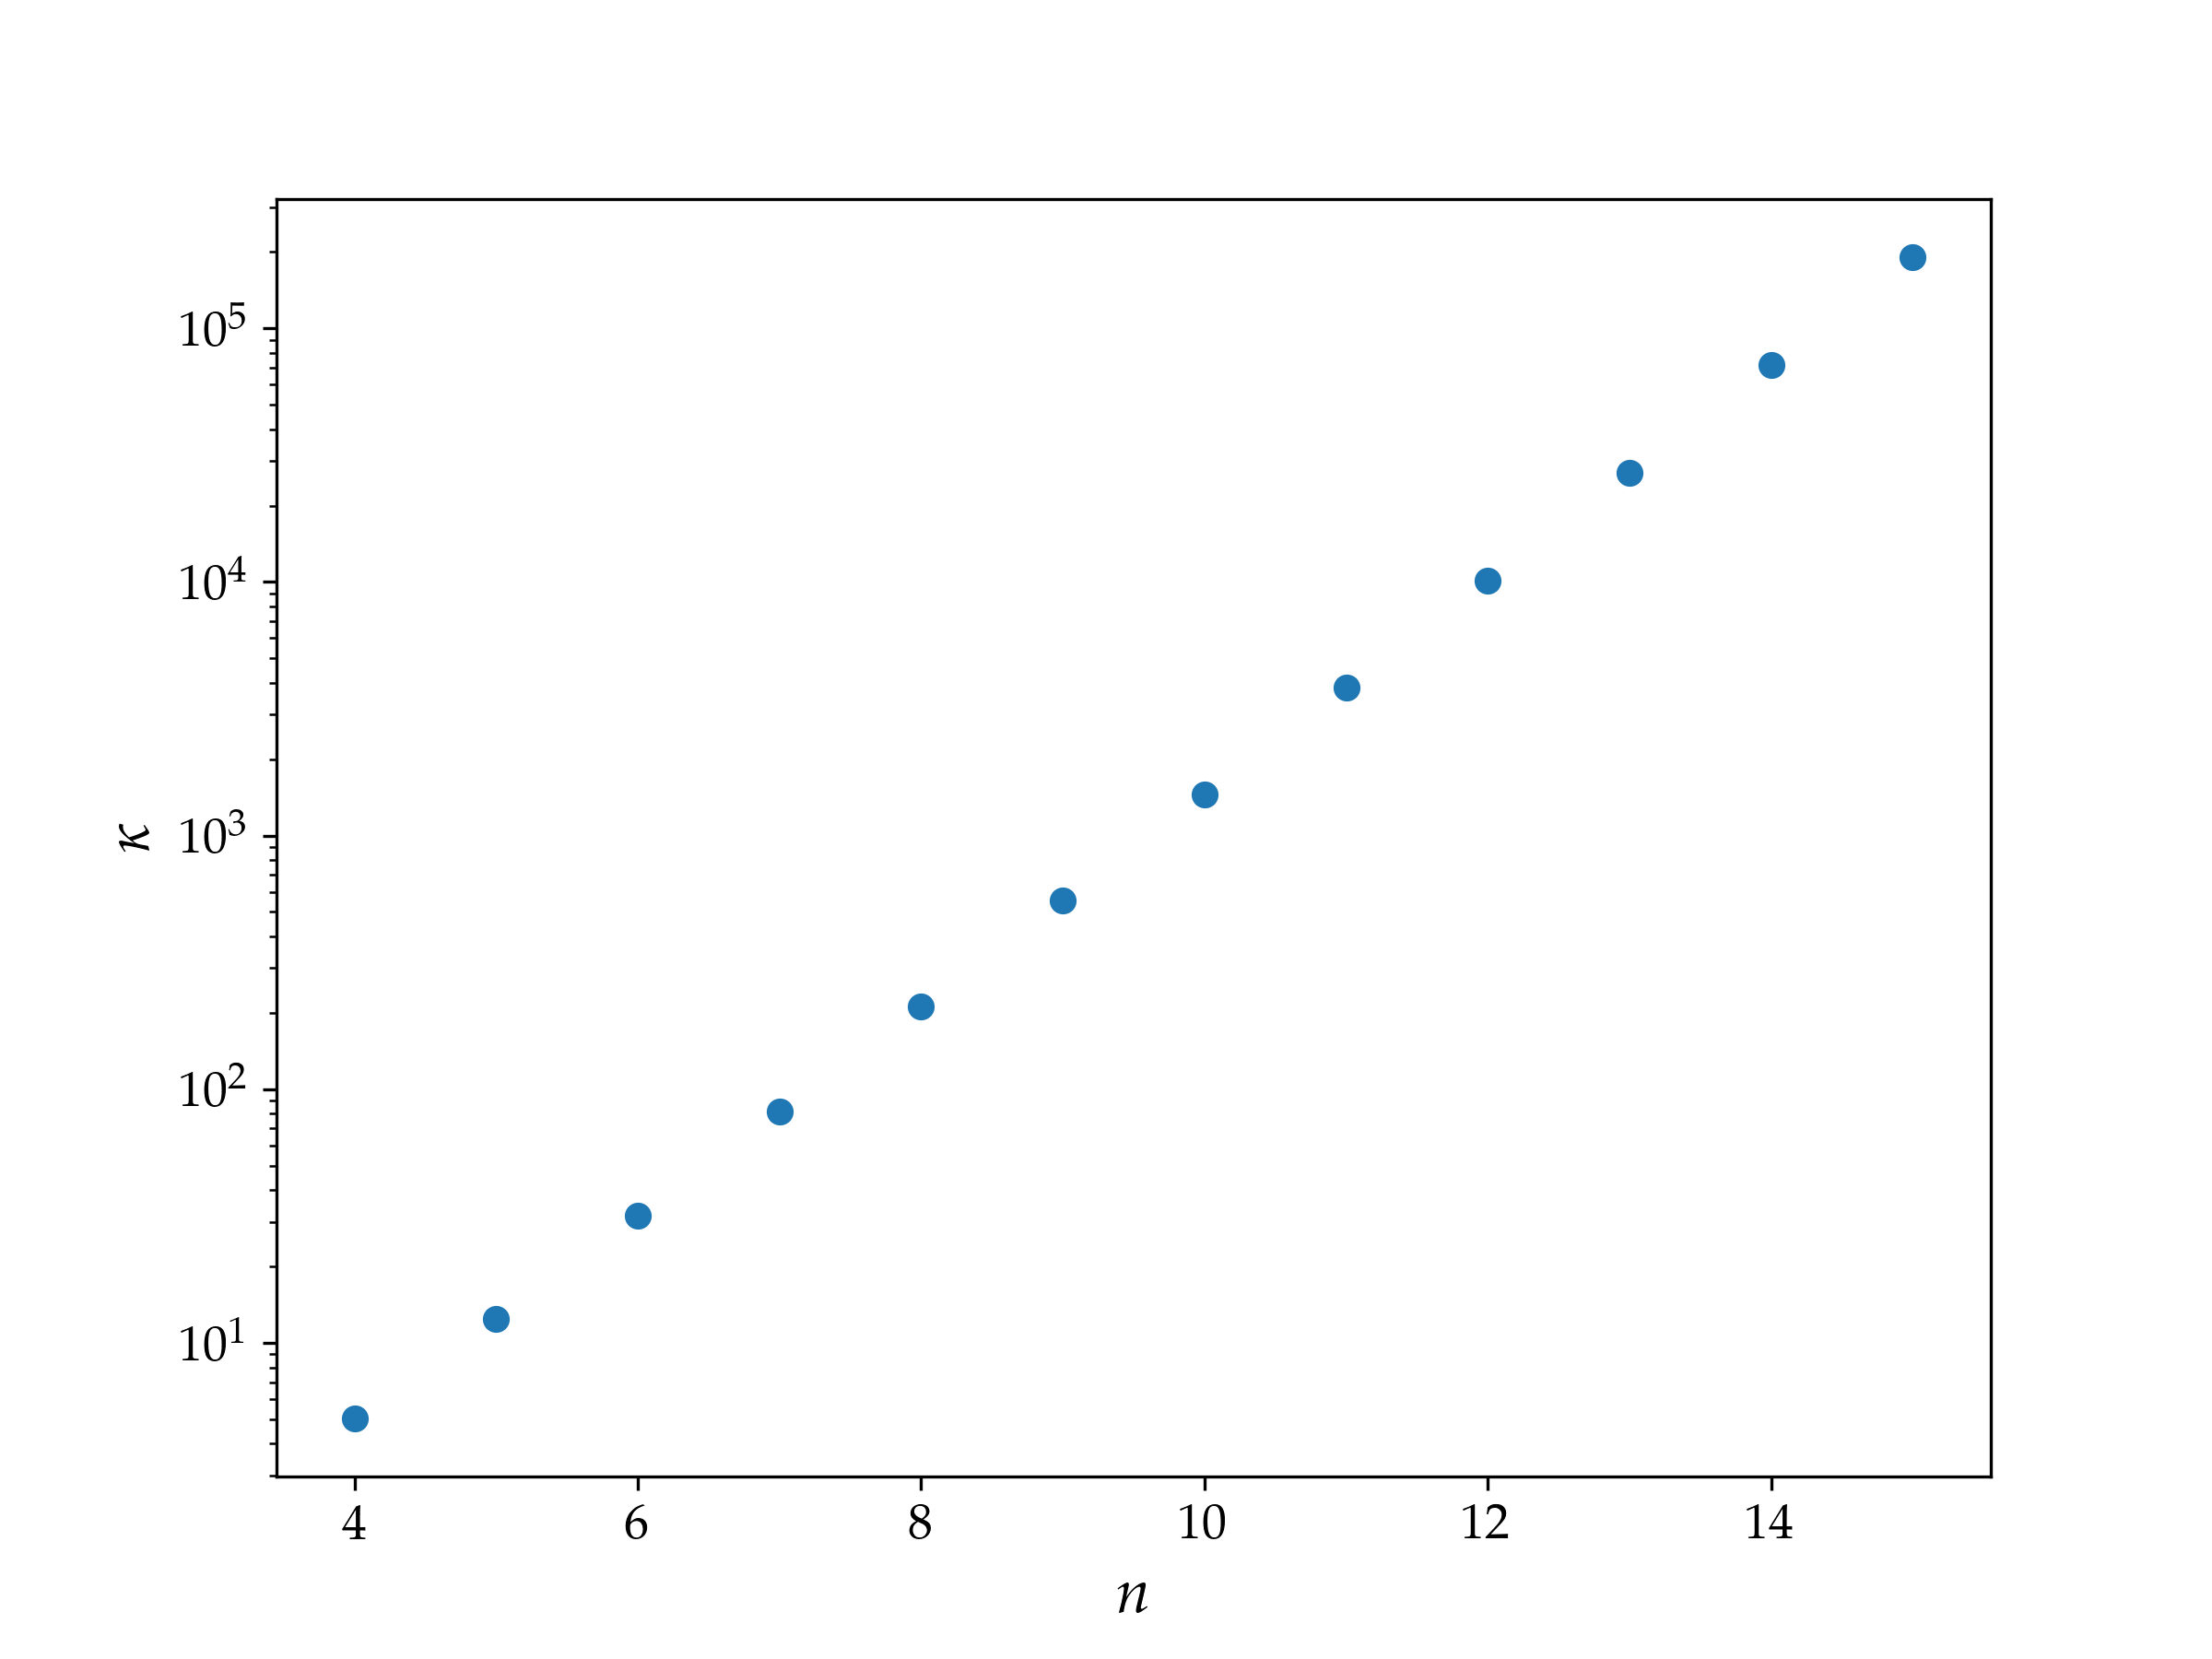
\includegraphics[width=0.7\linewidth]{images/8/Vandermonde_cond.png}
    \caption{\textit{Condition number} $\kappa$ della matrice di Vandermonde in funzione del numero di punti da interpolare $n$.}
    \label{fig: Vandermonde cond}
\end{figure}

\subsubsection{Lagrange Interpolation}
Un'alternativa è proposta dall'interpolazione di Lagrange, dove definiamo i \textit{Polinomi di Lagrange} $L_k(x)$:
\[
L_k(x) = \frac{\prod_{j=0, j \neq k}^{n-1}(x - x_j)}{\prod_{j=0, j \neq k}^{n-1}(x_k - x_j)} = w_k \prod_{j=0, j \neq k}^{n-1}(x - x_j)\
\]
\[
\frac{1}{w_k} = \prod_{j=0, j \neq k}^{n-1}(x_k - x_j) \quad \text{è una costante}
\]
La caratteristica principale di $L_k(x)$ è quella che 
\[
L_k(x_i) = \delta_{ki}
\]
quindi segue:
\[
P(x) = f = \sum a_k\ L_k(x) = \sum a_k \delta_{ki} = a_i
\]
Cioè la matrice di Vandermonde è l'identità, e non è necessario risolvere il sistema lineare poiché è banale. \\
Una riscrittura è possibile per ottimizzare il costo computazionale del problema:
\[
\begin{aligned}
P(x) = \dots = \left[ \sum_{k} \frac{f_k w_k}{(x - x_k)} \right] \left[ \sum_{k} \frac{w_k}{(x - x_k)} \right]^{-1}
\end{aligned}
\]

\noindent Si noti che nel calcolo del polinomio esattamente su un nodo si potrebbero incontrare problemi di divergenza del risultato numerico: risolviamo introducendo una piccola deviazione $\epsilon$, dell'ordine della \textit{machine precision}, trascurabile nel calcolo ordinario, ma che assicura alla nostra computazione, in questi casi più delicati, di non fallire

\[
\begin{aligned}
P(x) = \dots = \left[ \sum_{k} \frac{f_k w_k}{(x - x_k + \epsilon)} \right] \left[ \sum_{k} \frac{w_k}{(x - x_k + \epsilon)} \right]^{-1}
\end{aligned}
\]

\subsection{Risultati e Discussione}
L'uso di una classe risulta naturale, infatti il calcolo dei pesi è un'operazione da fare una sola volta, dato un certo set di punti, quindi essi possono essere computati e conservati.\\
Ho implementato questo tipo di logica nella mia soluzione:
\begin{elegantcode}
class Lagrange:
    def __init__(self, x, f):
        self.x = x
        self.f = f
        n = len(x)
        w_arr = []
        for k in range(n):
            mask = np.ones(len(x), dtype=bool)
            mask[k] = False
            wk = np.prod((x[k] - x[mask] + 1e-15))**(-1)
            w_arr.append(wk)
        self.w = np.array(w_arr)

    ...
\end{elegantcode}
\bigskip
\noindent Sono forniti 3 \textit{dataset}, vengono mostrati di seguito i punti nel piano (Fig \ref{fig: Repr dataset}) e la loro interpolazione con una curva, tramite metodo dei Polinomi di Lagrange (Fig \ref{fig: Lagrange interp}).

\begin{figure}[H]
    \centering
    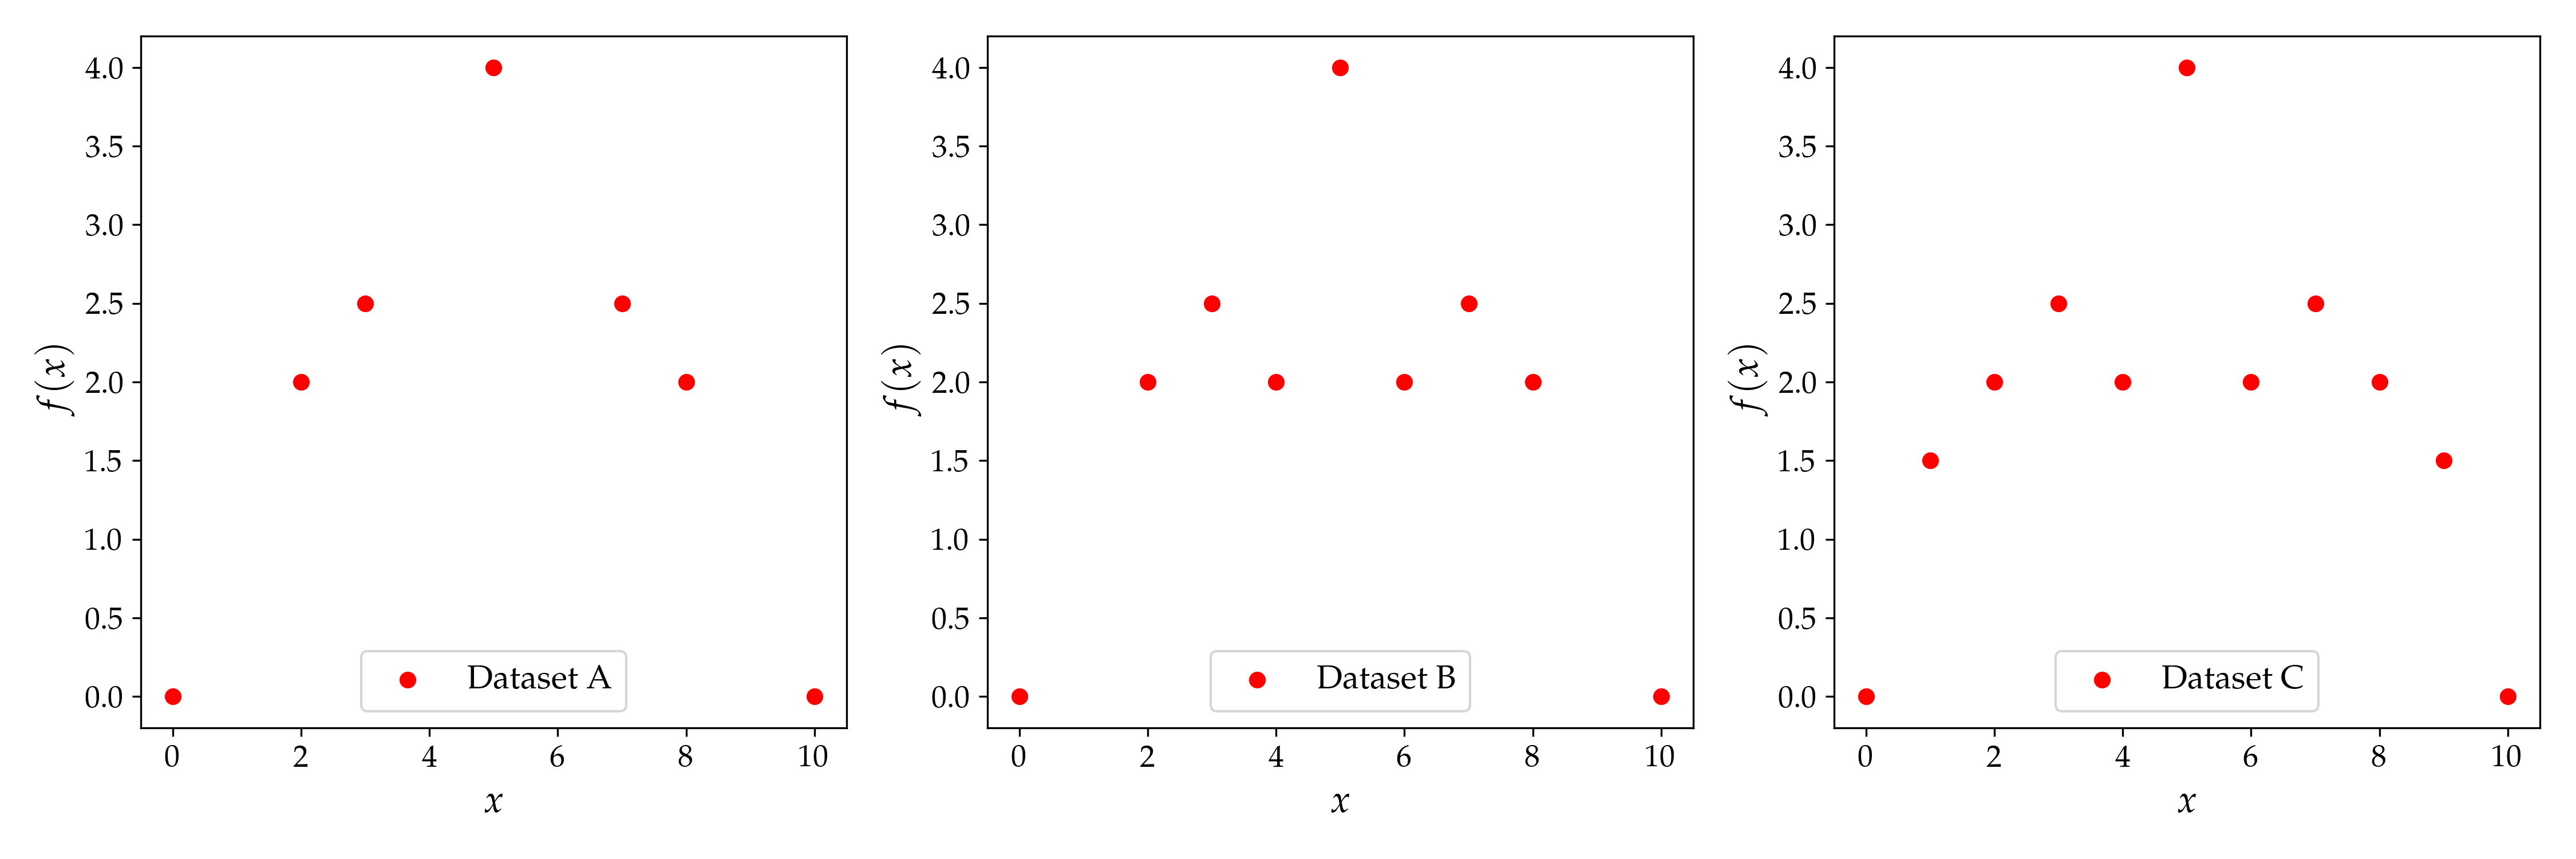
\includegraphics[width=\linewidth]{images/8/Lagrange_dataset_plot.png}
    \caption{Rappresentazione dei dataset.}
    \label{fig: Repr dataset}
\end{figure}

\begin{figure}[H]
    \centering
    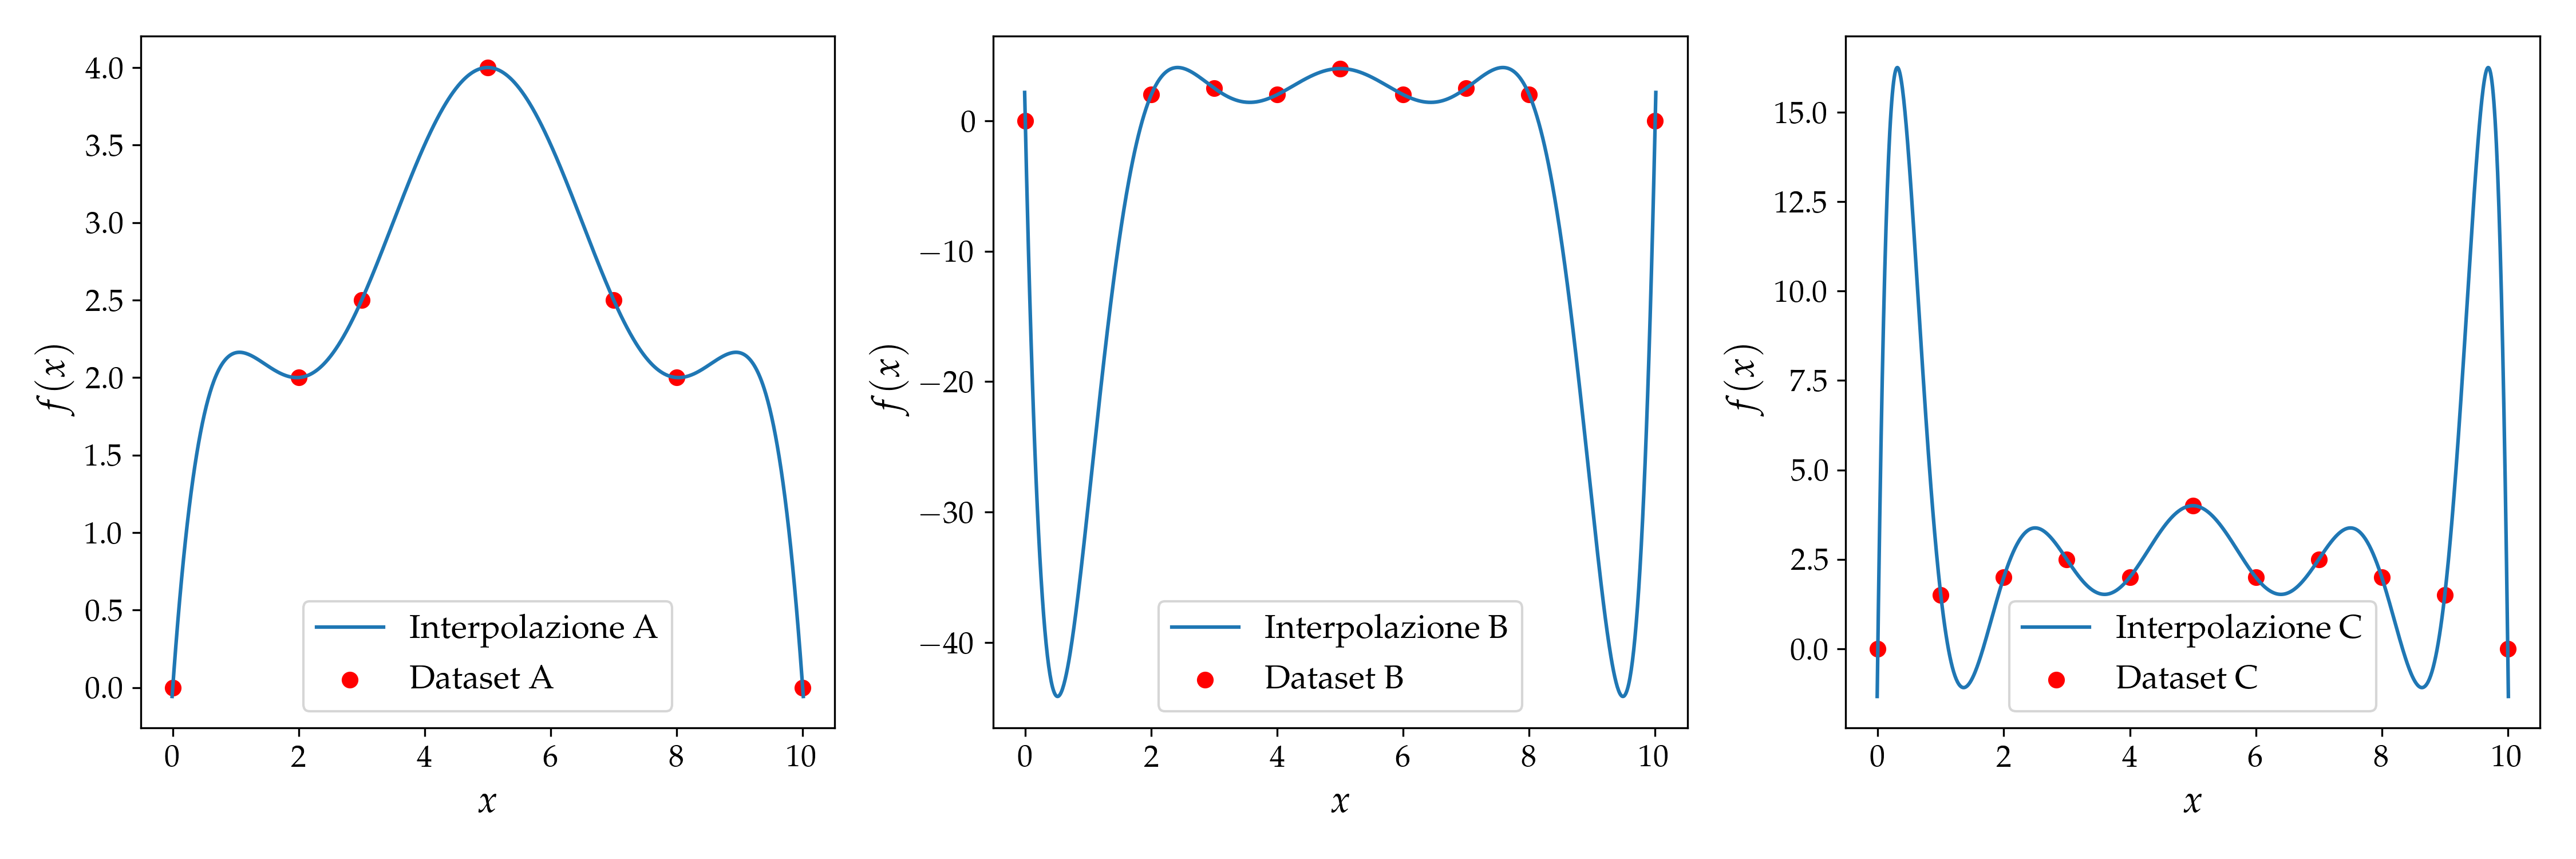
\includegraphics[width=\linewidth]{images/8/Lagrange_Interpolation.png}
    \caption{Interpolazione con \textit{Lagrange}.}
    \label{fig: Lagrange interp}
\end{figure}

\bigskip
\noindent Risulta interessante il confronto con l'interpolazione della curva tramite il \textit{Direct Method}. I problemi principali di questo approccio sono stati presentati nel Cap. \ref{Cap: Direct Mth}, ma qui vogliamo analizzare i risultati diretti di questa implementazione.

Nella Fig. \ref{fig: Dir mth interp} vediamo rappresentata la forma funzionale, polinomiale, trovata da questo secondo metodo e risulta evidente la similitudine con Fig. \ref{fig: Lagrange interp}.
\begin{figure}[H]
    \centering
    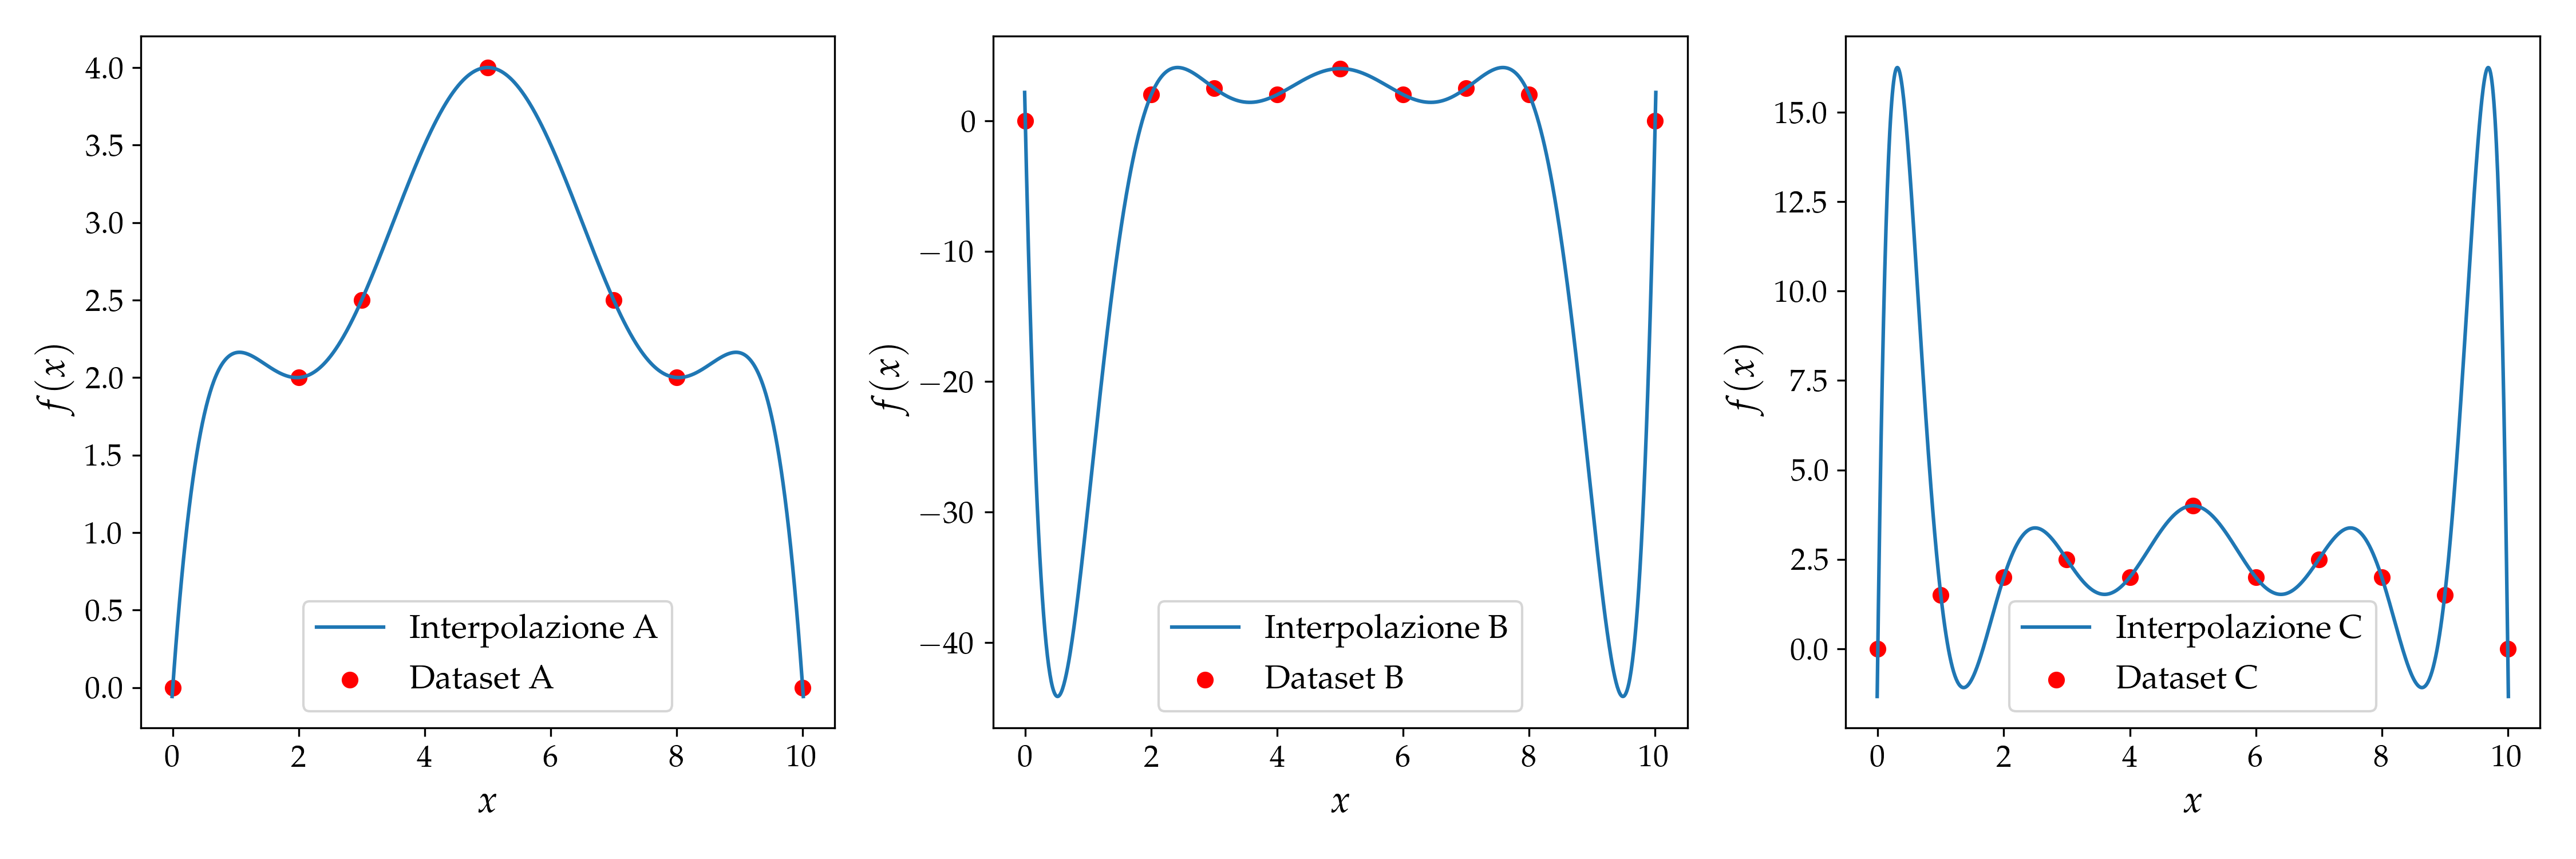
\includegraphics[width=\linewidth]{images/8/Direct_mth.png}
    \caption{Interpolazione con \textit{Direct Method}.}
    \label{fig: Dir mth interp}
\end{figure}

\noindent Una anlisi più precisa del fenomeno è possibile osservando l'errore assoluto tra le due descrizioni, definito come $|f_L(x) - f_D(x)|= E(x)$. Con riferimento al plot in Fig. \ref{fig: Err dir vs lag}, possiamo descrivere due andamenti differenti: se in prima analisi si osserva empiricamente una correlazione qualitativa tra l’andamento dell’errore e quello della funzione (ma senza una relazione generale), esiste un secondo \textit{slope} più interessante e preponderante nella parte destra del grafico. 

\medskip
\noindent Si osserva che $E(x)$ passa da un andamento regolare e ben definito a uno caratterizzato da oscillazioni sempre più pronunciate. Inoltre, l’ordine di grandezza dell’errore aumenta all’aumentare del numero di punti, mostrando una crescita approssimativamente esponenziale.

La spiegazione per queste osservazioni viene trovata nel mal condizionamento della \textit{Matrice di Vandermonde} e nel \textit{Direct Method}. Abbiamo mostrato già nel Cap.\ref{Cap: Direct Mth} come al crescesere del numero di punti, aumenti $\kappa$ per $V$, e questo spiega i diversi ordini di grandezza visibili sulla scala degli errori per i differenti dataset. 

Per quanto riguarda le oscillazioni della funzione, è necessario ricondursi alla definizione della matrice $V$, che contiene, nelle ultime colonne, termini dell'ordine di $x_i^N$, con $N$ numero di punti. Per N grande vengono molto amplificati gli errori sui coefficienti (instabilità numerica), inoltre le combinazioni di potenze con coefficienti di segno opposto porteranno a somme algebriche di numeri con diversi ordini di grandezza di differenza: questo lascia la possibilità per errori di arrotondamento legati alla \textit{machine precision}.

\medskip
\noindent Infine si può notare come spesso i minimi dell'errore si trovino in corrispondenza dei nodi, cioè dei punti in cui fissiamo il valore della funzione in maniera più rigida: le due interpolazioni saranno tendenzialmente più concordi sui valori qui assegnati.

\begin{figure}[H]
    \centering
    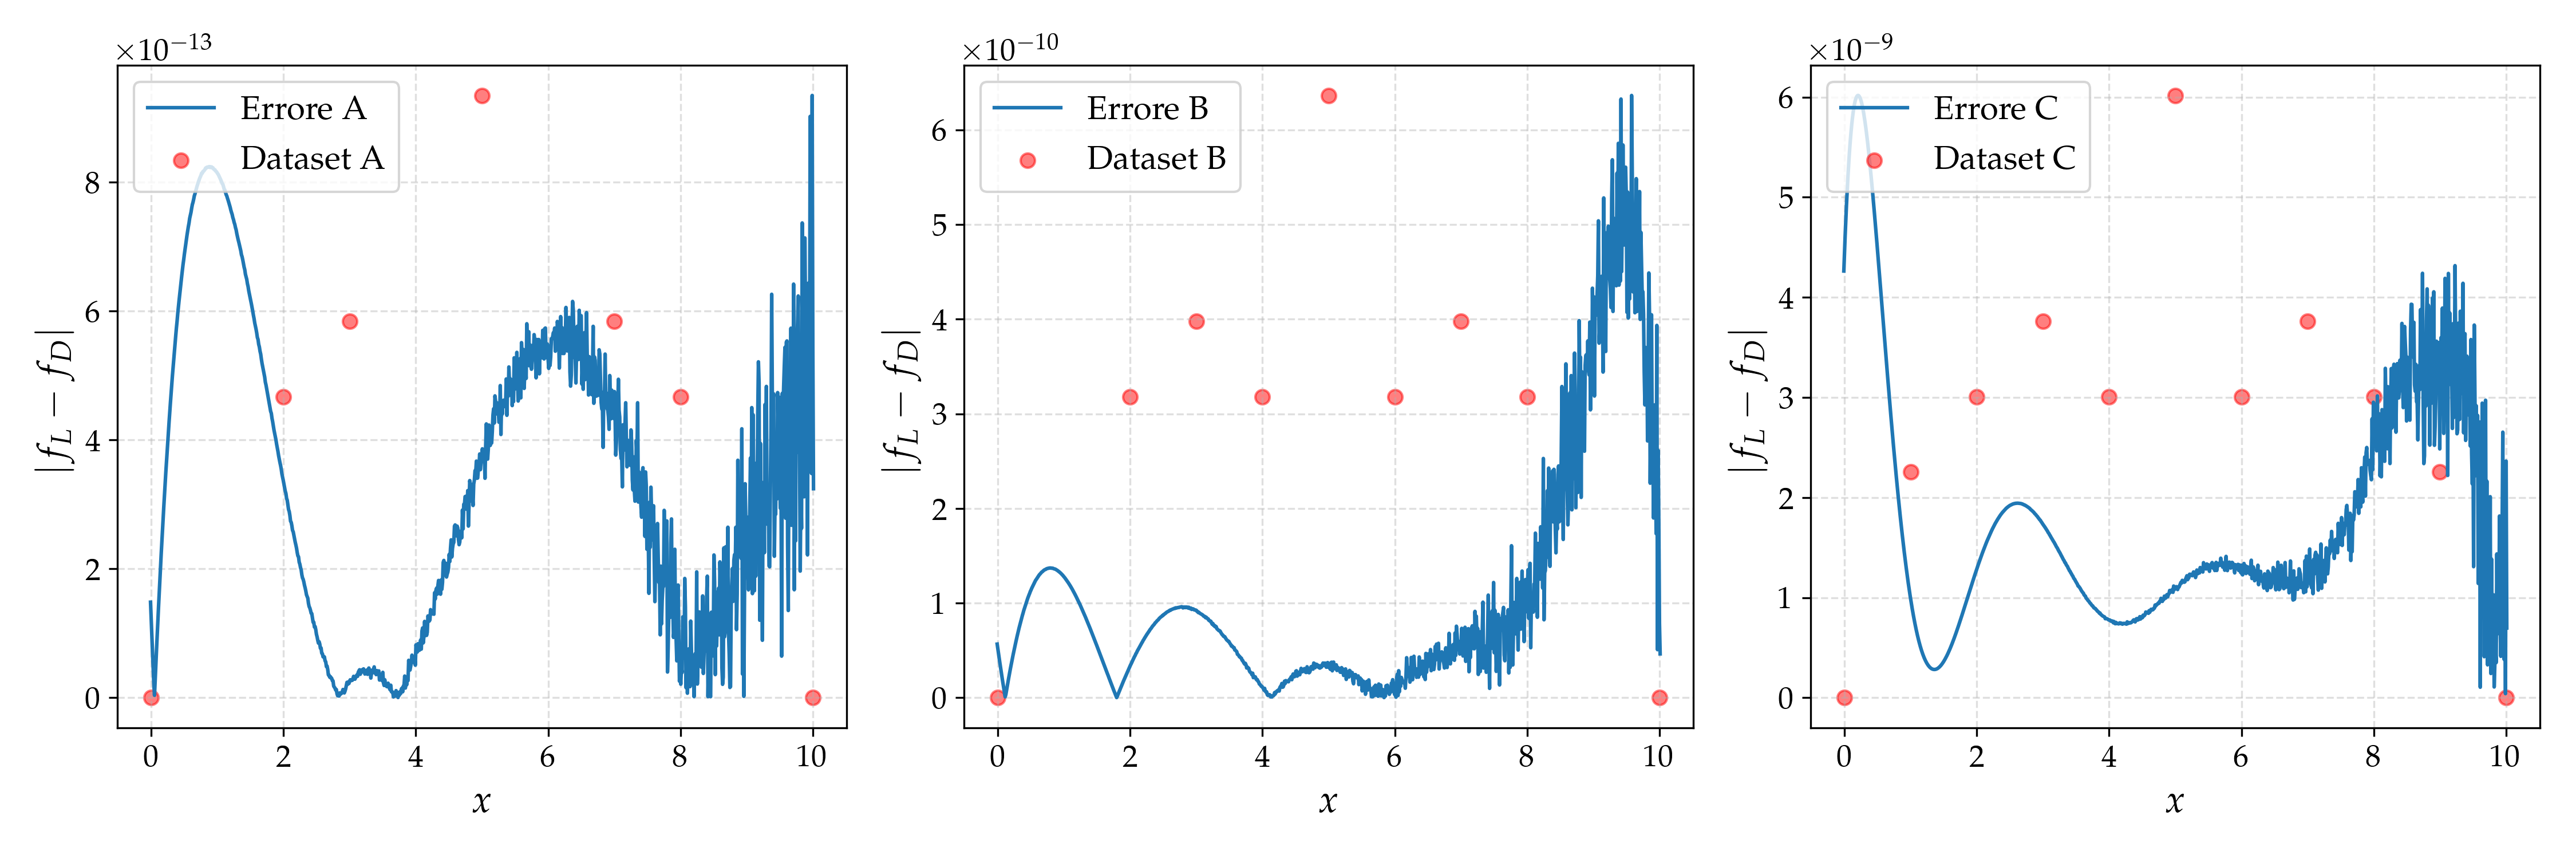
\includegraphics[width=\linewidth]{images/8/Err_dir_vs_lag.png}
    \caption{Plot dell'errore assoluto tra i metodi di \textit{Lagrange Interpolation} e \textit{Direct Method}, sui differenti dataset definiti in Fig. \ref{fig: Repr dataset}, che sono rappresentati in sovraimpressione, normalizzati per essere confrontabili con le dimensioni dell'errore.}
    \label{fig: Err dir vs lag}
\end{figure}
\newpage





\section{Esercizio 4.2.1}
\subsection{Problem Statement}
Si consideri la funzione di Runge
\[
\frac{1}{1 + 25x^2}.
\]
nel’intervallo $I=[-1,1]$. Calcolare la funzione interpolante utilizzando $N = 10, 20, 30, 40, 50$ nodi definiti sia come nodi equispaziati sia come nodi di Chebyshev. Utilizzare l’interpolatore basato sui polinomi di Lagrange e la \textit{monomial basis} (\textit{direct method} tramite matrice di Vandermonde).

\subsection{Premessa Teorica}
Nel contesto dell'interpolazione polinomiale di punti risulta interessante valutare le conseguenze date dal \textit{\textbf{Teorema di Stone-Weierstrass}}, che ci portano ad affermare che:
\begin{quote}
    ``Per un'interpolazione polinomiale, aumentando il numero di punti, cioè il grado del polinomio, è possibile aumentare anche l'accuratezza.''
\end{quote}

\noindent Ciò però non ci dice quale sia il metodo migliore nè stabilisce che tutti gli algoritmi siano equivalenti; l'esempio della funzione di Runge ci permette di mostrare l'efficacia di un modello diverso da quello utilizzato fin'ora negli esempi che abbiamo presentato. Si può mostrare come la scelta del sampling non uniforme con i \textit{nodi di Chebyschev} rappresenta un esempio di metodo che permette di risolvere il fenomeno di Runge.
 
\subsection{Metodi Numerici e Algoritmi}

\medskip
\noindent La funzione di Runge è definita come:
\[
f(x) = \frac{1}{1 + 25x^2}.
\]
ed è possibile mostrare come, per questo esempio, l'accuratezza della funzione interpolata, in $I$, diminuisca rispetto al modello al crescere del numero di punti che campioniamo, se scegliamo un campionamento uniforme. 

Un esempio in Fig. \ref{fig: Lag unif} dove il numero di nodi (uniformi) varia nell'intervallo $[10, 60]$ ed è possibile osservare come solo nell'intorno del massimo si migliori l'accuratezza; verso gli estremi accade il contrario, in maniera che la differenza con $f(x)$ sia assolutamente non trascurabile. 
Se definiamo i \textit{nodi di Chebyschev} come:
\[
x_j = -\cos \left( \frac{j\pi}{n-1} \right) \quad j = 0, 1 \dots n-1
\]
cioe come punti equidistanti su una circonferenza unitaria, ma proiettati sul suo diametro. Si può dimostrare che questo diventa un migliore sampling per l'intervallo $I$, come mostra il confronto con la Fig. \ref{fig: Lag Cheby}. I nodi di Chebyshev riducono l’errore massimo e, per funzioni regolari, favoriscono la convergenza dell’interpolante.

 \begin{figure}[H]
     \centering
     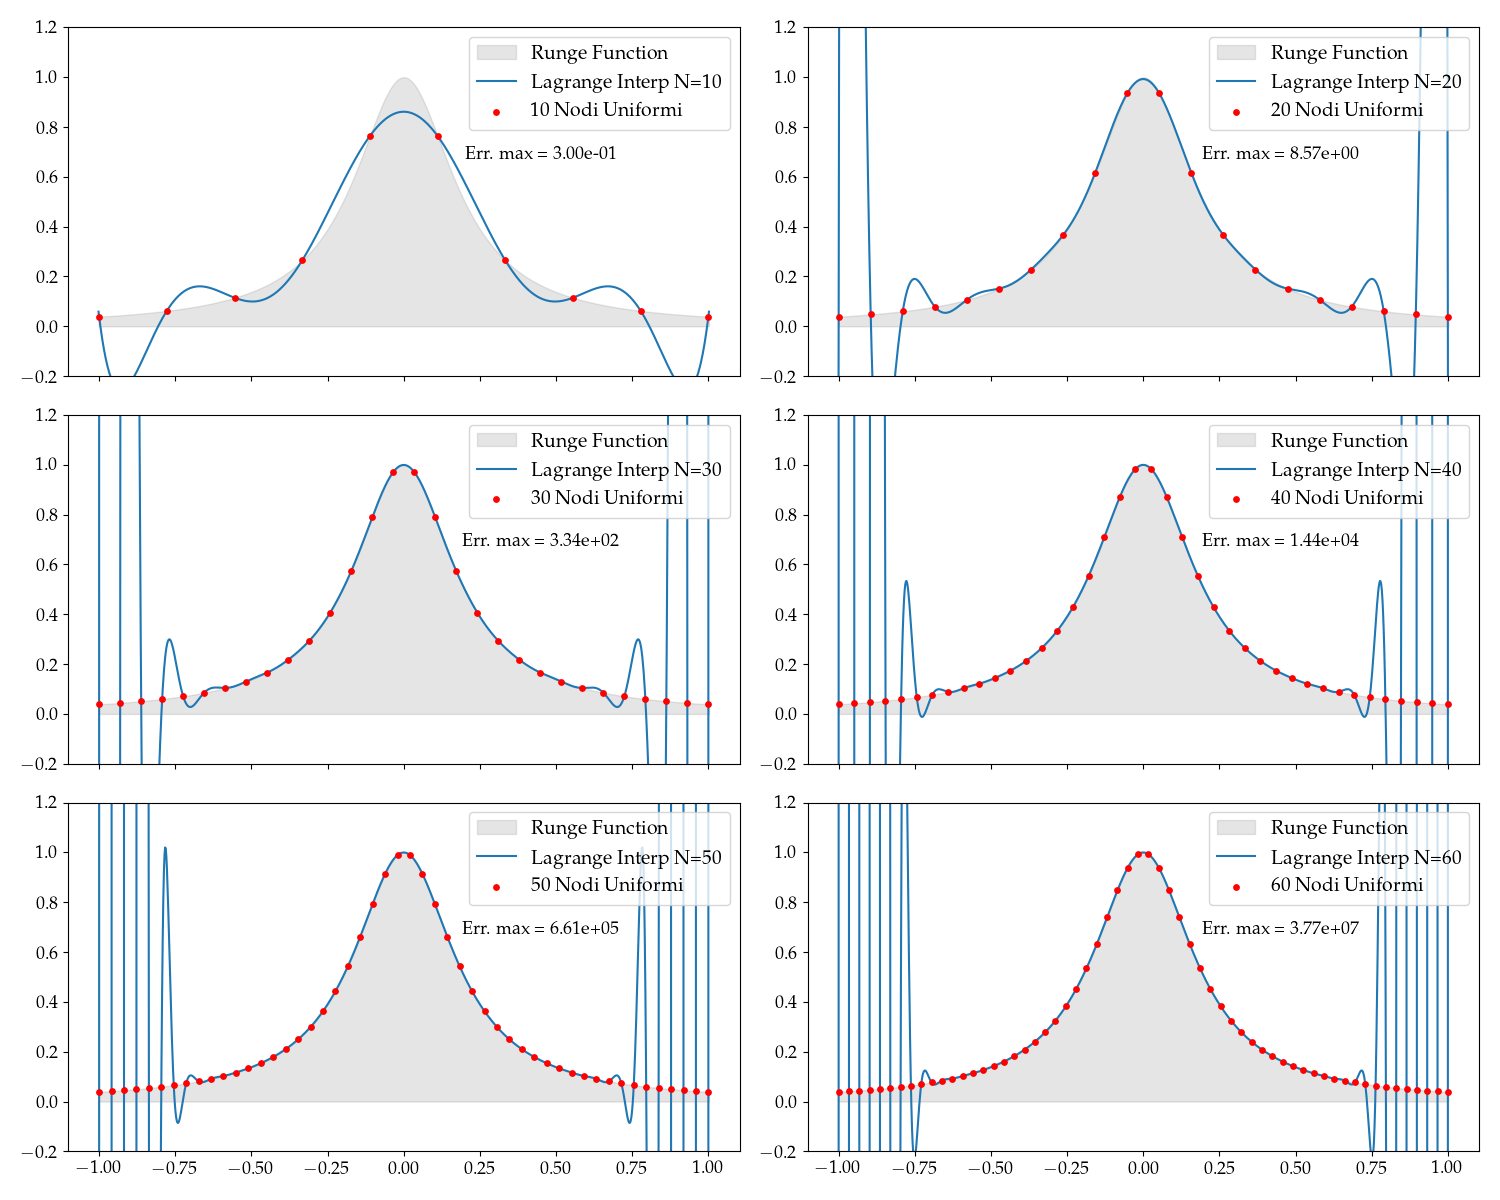
\includegraphics[width=\linewidth]{images/9/lagr_unif.png}
     \caption{\textit{Lagrange interpolation} di $f(x)$ in $[-1,1]$, nodi uniformi.}
     \label{fig: Lag unif}
 \end{figure}

\begin{figure}[H]
    \centering
    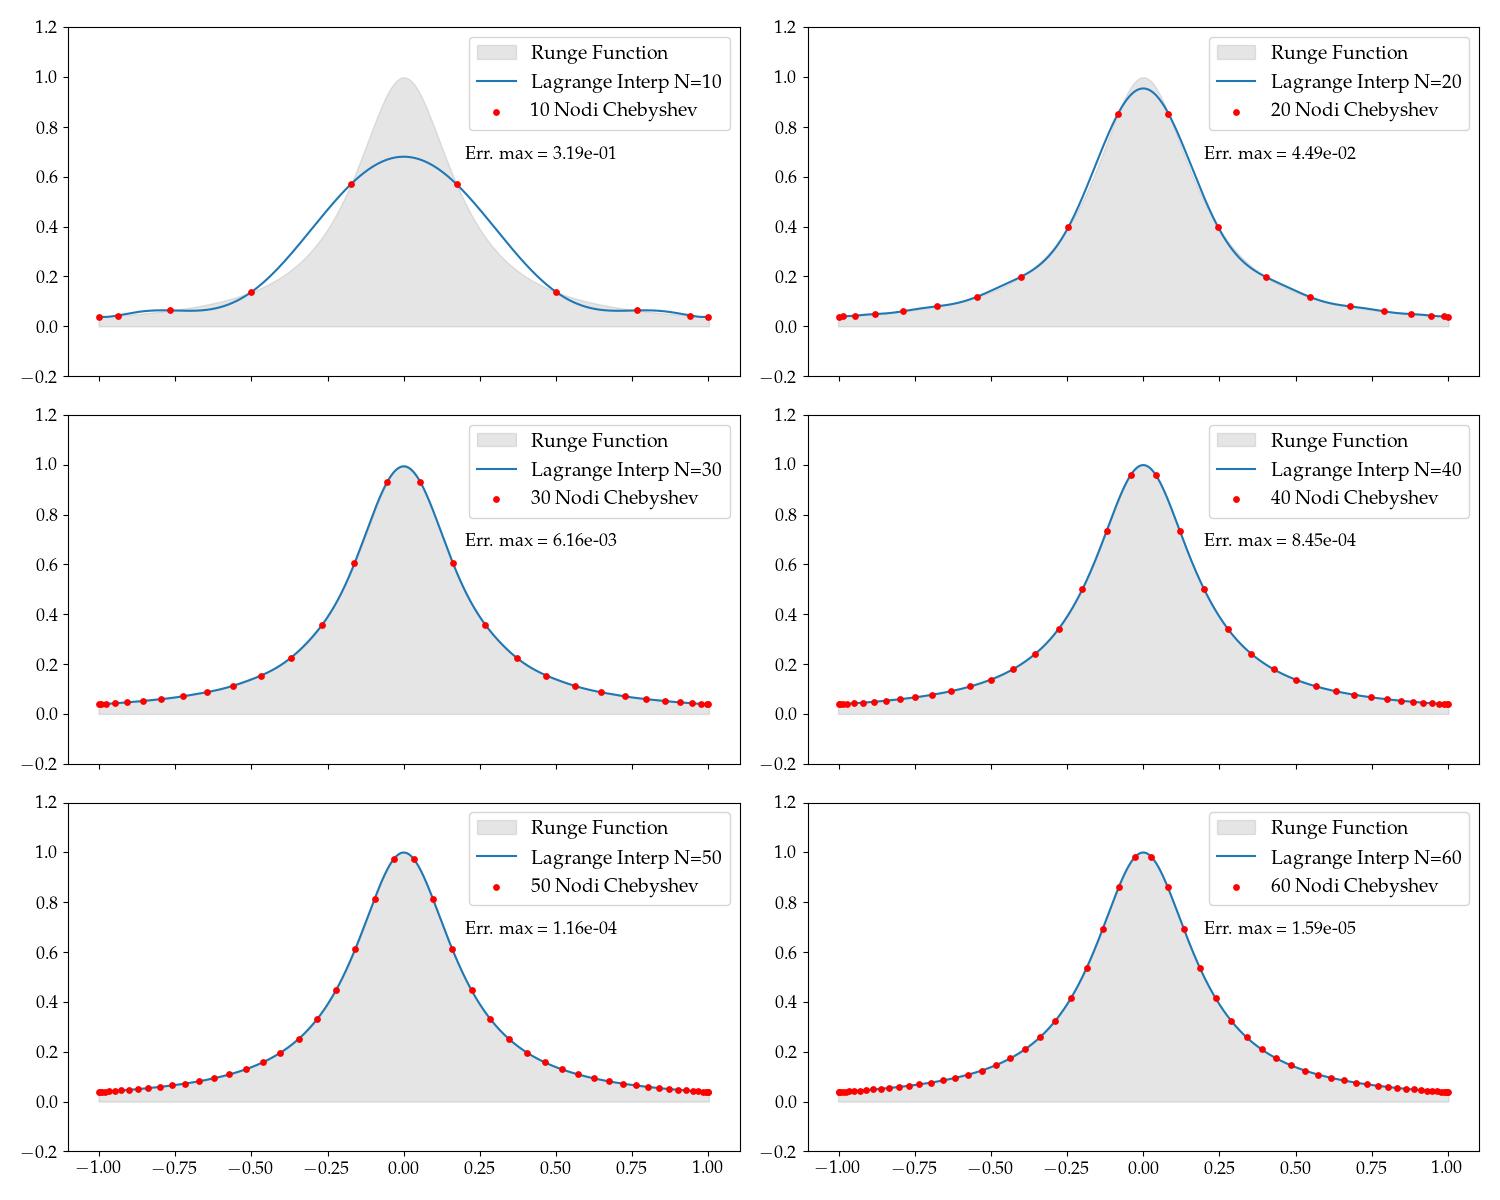
\includegraphics[width=\linewidth]{images/9/lagr_cheby.png}
    \caption{\textit{Lagrange interpolation} di $f(x)$ in $[-1,1]$, nodi di Chebyschev.}
    \label{fig: Lag Cheby}
\end{figure}
     
\subsection{Risultati e Discussione}
Le figure che abbiamo mostrato sottolineano la praticità e correttezza dell'utilizzo del sampling dei \textit{nodi di Chebyschev} per un algoritmo di intepolazione più accurato. \noindent Nelle stesse figure a cui avevamo fatto riferimento, indicato in sovraimpressione, abbiamo anche l'errore massimo nei nodi, nel confronto con $f(x)$: si osserva numericamente, nei plot di Fig. \ref{fig: Lag unif err} e Fig. \ref{fig: Lag cheby err} una crescita molto rapida (quasi esponenziale) che si ha all'aumentare del numero di nodi uniformi interpolanti, mentre un fenomeno opposto con i nodi di Chebyschev. 

\begin{figure}[H]
    \centering
    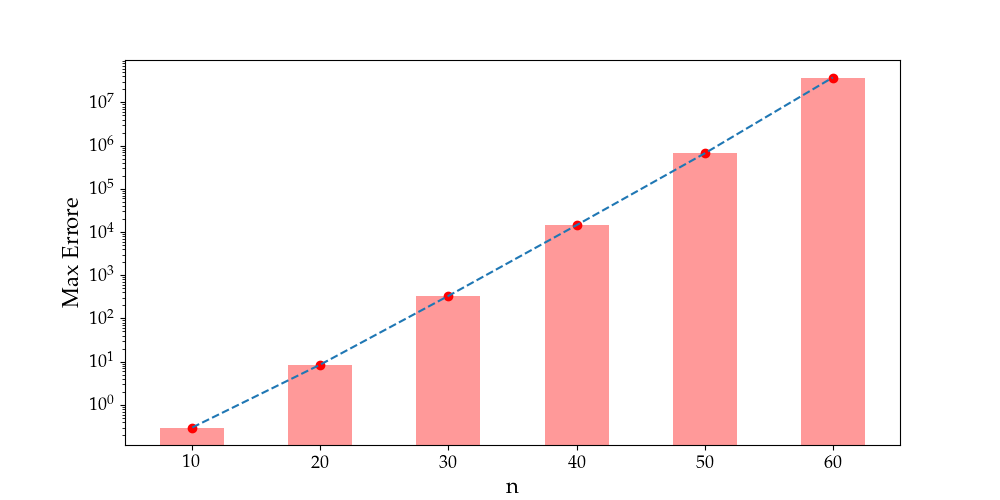
\includegraphics[width=0.8\linewidth]{images/9/unif_err.png}
    \caption{Errore massimo della funzione interpolata al variare del numero di nodi uniformi: è possibile osservare come l'\textit{Err Max} aumenti in maniera esponenziale, usando questo metodo.}
    \label{fig: Lag unif err}
\end{figure}

\begin{figure}[H]
    \centering
    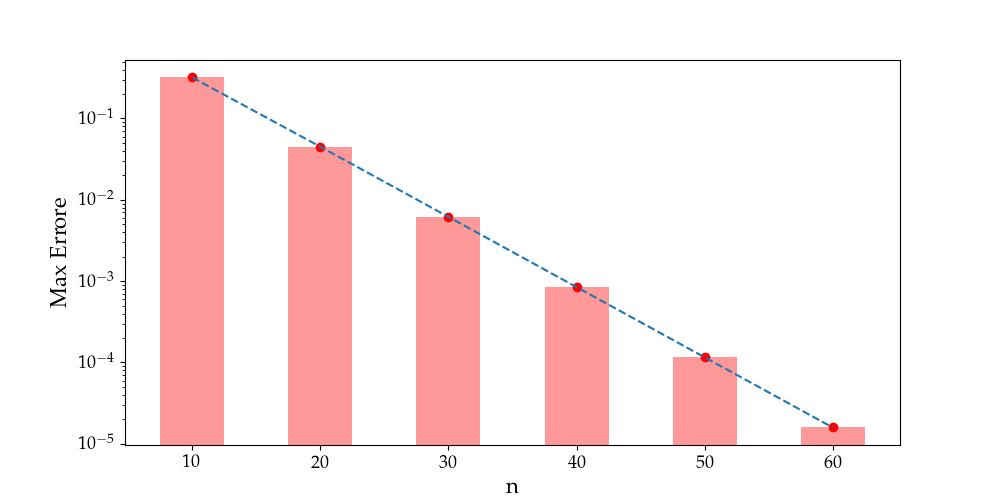
\includegraphics[width=0.8\linewidth]{images/9/cheby_err.png}
    \caption{Errore massimo della funzione interpolata al variare del numero di nodi di Chebyschev: vi è una decrescita esponenziale.}
    \label{fig: Lag cheby err}
\end{figure}

\noindent Infine ci interessa sottolineare che questo fenomeno non è proprio del metodo di interpolazione che abbiamo scelto, che per gli esempi precedenti era stato la \textit{Lagrange Interpolation}, difatti possiamo mostrare come anche per un metodo alternativo, scegliamo il \textit{Direct method}, è possibile mostrare lo stesso fenomeno di Runge.

\begin{figure}[H]
    \centering
    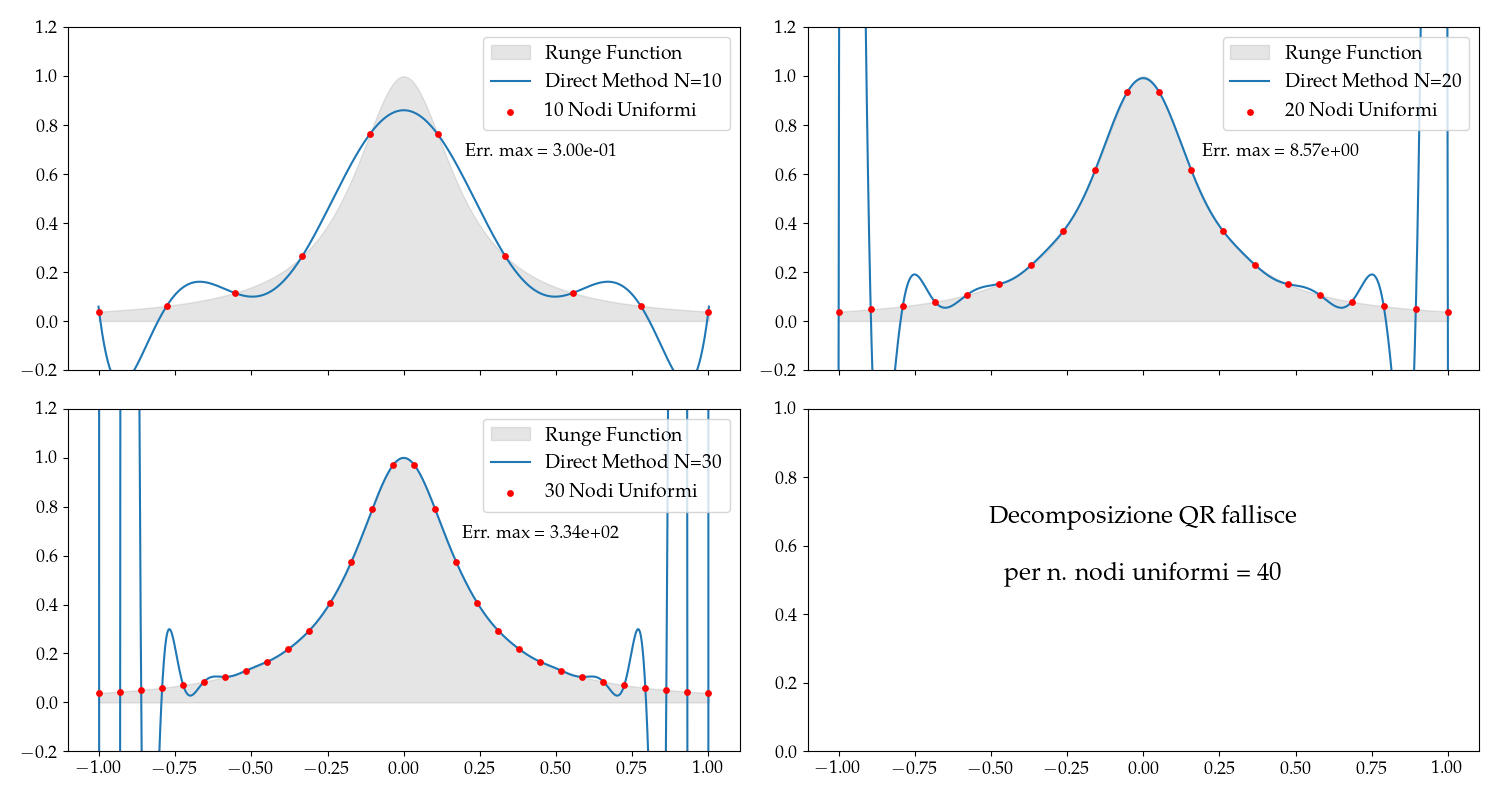
\includegraphics[width=0.8\linewidth]{images/9/direct_unif.png}
    \caption{\textit{Direct method} su $f(x)$ in $[-1,1]$, nodi uniformi. Sono note dal Cap. \ref{Cap: Direct Mth} le problematiche di questo metodo di interpolazione, che risultano più evidenti all'aumentare del numero di nodi: il risultato diventa numericamente instabile per $n \gtrsim 40$ a causa del mal condizionamento della matrice di Vandermonde.”}
    \label{fig: Direct unif}
\end{figure}

\begin{figure}[H]
    \centering
    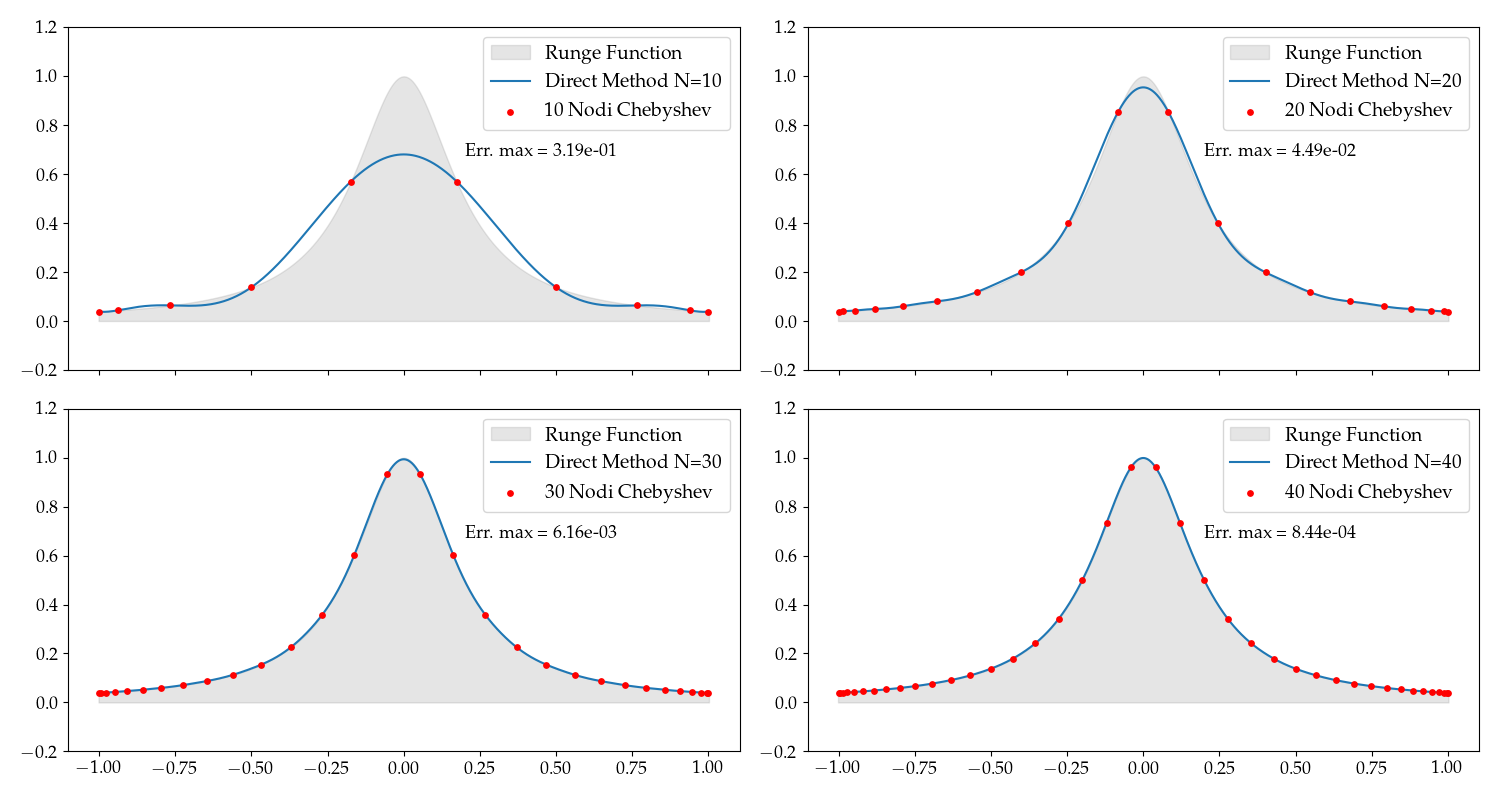
\includegraphics[width=0.8\linewidth]{images/9/direct_cheby.png}
    \caption{\textit{Direct method} su $f(x)$ in $[-1,1]$, nodi Chebyschev. Il metodo fallisce per $n \gtrsim 50$.}
    \label{fig: Direct cheby}
\end{figure}

\newpage








\section{Esercizio 4.4.1}
\subsection{Problem Statement}
Scrivi una classe che, dato l'insieme discreto di coordinate $x_i$, calcoli e memorizzi la matrice $W_{ij}$. 
Aggiungi i metodi \texttt{dft} e \texttt{idft}, entrambi i quali accettano un array della stessa lunghezza di $\{x_i\}$ 
e restituiscono la DFT diretta o inversa (internamente i due metodi applicano 
la matrice $W$ o la sua aggiunta $W^\dagger$). Partendo dai seguenti parametri:
\begin{itemize}
    \item $L = 2\pi$
    \item $N = 128$
    \item $\alpha = 0.5$
    \item $u(x, 0) = \sin(x) + 0.5 \sin(3x)$
\end{itemize}

\noindent Risolvi l'equazione del calore 1D implementando questi passaggi:
\begin{enumerate}
    \item Applica la DFT diretta a $u(x, 0)$ e calcola $\tilde{u}(k, 0)$
    \item Calcola $\tilde{u}(k, t)$
    \item Applica la DFT inversa a $\tilde{u}(k, t)$ per trovare $u(x, t)$
\end{enumerate}

\noindent Ripeti questa operazione per 20 valori di $t \in [0, 2]$ e poi plottali insieme.

\subsection{Premessa Teorica}
\subsubsection{Interpolazione Trigonometrica}
nei capitoli precedenti ci siamo occupati di interpolazioni lineari, cioè in cui vale che:
\[
P(x) = \sum a_k \phi_k(x)
\]
in particolare scegliendo $\phi_k(x) = x^k$, cioè definendo un'interpolazione polinomiale. Un'alternativa a questo approccio è data da un'interpolazione trigonometrica, cioè in cui $\phi_k(x) = e^{ikx} = \omega^k, \quad \omega = e^{ix}$. Questa diventa un'estensione complessa della base dei monomi, permettendo di estendere anche il teorema di unicità, che affermava:

\bigskip
\noindent Dato l'insieme di $N$ punti $x_k = 2\pi k/N$, con $k = 0, 1 \dots N - 1$, per ogni insieme di punti di supporto $(x_k, f_k)$, con $f_k$ complesso, esiste un unico polinomio

\[
P(x) = \sum_{k=0}^{N-1} a_k e^{ikx}
\]

\noindent che soddisfa $P(x_k) = f_k$ per ogni $k$. Definendo $\omega_k = e^{ix_k} = e^{2\pi i k/N}$, i coefficienti possono essere calcolati esplicitamente utilizzando

\[
a_k = \frac{1}{N} \sum_{j=0}^{N-1} f_j \omega_j^{-k} = \frac{1}{N} \sum_{j=0}^{N-1} e^{-2\pi ijk/N} f_j
\]

\noindent In genere, i coefficienti $a_k$ sono chiamati la trasformata di Fourier di $f$ e vengono indicati con $\tilde{f}_k$.
Definendo $\Delta x = L/N$, cioè il passo di sampling regolare su un intervallo $[0, L]$, definiamo la \textit{Trasformata di Fourier diretta} (DFT):
\[
\tilde{f}(p) = \Delta x \sum_{i=0}^{N-1} f(x_i) e^{ipx_i}
\]
dove p è il momento, cioè la coordinata nello spazio di Fourier. La trasformata inversa (IDFT) diventa quindi:
\[
f(x_i) = \frac{1}{L} \sum_{j=0}^{N-1} e^{-ip_j x_i} \tilde{f}(p_j)
\]

\subsubsection{Equazione del calore 1D}
In particolare la FT ci viene in aiuto come metodo standard per risolvere alcuni tipi di equazioni differenziali: nello spazio dei momenti la derivata rispetto alle coordinate diventa un semplice prodotto, semplificando molto il calcolo, in particolare consideriamo l'equazione del calore 1D su un dominio $x \in [0, L]$ con condizioni al contorno periodiche:

\begin{equation} \label{eq: Heat eq}
\frac{\partial u}{\partial t} = \alpha \frac{\partial^2 u}{\partial x^2}, \quad u(x, 0) = f(x)
\end{equation}

\begin{itemize}
    \item $u(x, t)$ è la temperatura alla posizione $x$ e al tempo $t$,
    \item $\alpha$ è la diffusività termica,
    \item $f(x)$ è la distribuzione iniziale di temperatura.
\end{itemize}

se valutiamo la trasformata del lato sx e dx:
\begin{itemize}
    \item $\mathcal{F} \left[ \frac{\partial u}{\partial t} \right] = \frac{\partial \tilde{u}}{\partial t}$
    \item $\mathcal{F} \left[ \frac{\partial^2 u}{\partial x^2} \right] = -p^2 \tilde{u}$
\end{itemize}

quindi l'equazione si riduce ad una ODE:
\[
\frac{\partial \tilde{u}}{\partial t} = -\alpha p^2 \tilde{u}
\]

la cui soluzione analitica è:
\[
\tilde{u}(p,t) = \tilde{u}(p,0) e^{-\alpha p^2t}
\]
La condizione sul valore iniziale è nota, risulta sufficiente calcolare la trasformata del valore iniziale; abbiamo quindi la soluzione nello spazio dei momenti, basta una IFT per tornare nello spazio delle coordinate e risolvere Eq. \ref{eq: Heat eq}
\[
\tilde{u}(p,t) \longrightarrow u(x,t)
\]

\subsection{Metodi Numerici e Algoritmi}
Per implementare la risoluzione del problema proposto risulta naturale passare ad una espressione matriciale della definizione della DFT e IDFT:
\[
\tilde{f}_k = \Delta x \sum_{i} W_{ki} f_i \quad \quad W_{ki} = e^{i p_k x_i}
\]
Questo offre la possibilità di usare gli algoritmi già sviluppati per la risoluzione dei sistemi lineari, in più permette un semplice passaggio da DFT a IDFT, che necessiterebbe di invertire $W$, ma che diventa il banale calcolo di $W^\dagger$:
$$W^\dagger W = N I \implies W^{-1} = \frac{1}{N} W^\dagger \implies W^\dagger = N W^{-1}$$
quindi:
\[
\tilde{f}_k = \Delta x \sum_{i} W_{ki} f_i \quad \quad f_i = \frac{1}{L} \sum_{k} W^\dagger_{ik} \tilde{f}_k 
\]

\medskip
\noindent Questa la classe che abbiamo implementato nel nostro codice \textit{.py}:
\begin{elegantcode}
class DFT:
    def __init__(self, x_desc):
        N = len(x_desc)
        L = (x_desc[-1] - x_desc[0])
        
        if N % 2 == 0: 
            p_pos = np.arange(N//2+1)   # positive values bcs of Niquist (even)
            p_neg = np.arange(1, N - (N//2)) * (-1)
        else: 
            p_pos = np.arange(N//2)     # positive values bcs of Niquist (odd)
            p_neg = np.arange(1, N - (N//2)) * (-1)

        p = 2 * np.pi / L * np.concatenate((p_pos, p_neg))
        W = np.exp(1j * np.outer(p, x_desc))

        self.W = W
        self.p = p
        self.N = N
        self.L = L
        self.dx = L / N
    
    def dft(self, y_desc):
        if type(y_desc)==int or len(y_desc) != self.N:
            raise ValueError('len(y_desc) must be equal to len(x_desc)!')
        y_dft = self.dx * self.W @ y_desc
        return y_dft

    def idft(self, y_desc):
        if type(y_desc)==int or len(y_desc) != self.N:
            raise ValueError('len(y_desc) must be equal to len(x_desc)!')
        y_idft = self.L**(-1) * self.W.conj().T @ y_desc
        return y_idft
    
\end{elegantcode}

\subsection{Risultati e Discussione}
L'esercizio permette un'efficace rappresentazione grafica tramite la libreria \textit{matplotlib}, in particolare con l'uso di mappe di colore e curve di livello, che esprimono il variare della $u(x,t)$. Sono mostrate due rappresentazioni differenti del fenomeno: in Fig. \ref{fig: Heat 2d} è dato un plot in cui segnamo diverse curve di livello, corrispondenti ai 20 valori temporali per cui valutiamo la funzione, ogni curva ha assegnato un colore, proprio di un valore temporale. In Fig. \ref{fig: Heat 3d} la rappresentazione è 3d, dove lungo l'asse x e y troviamo $x$ e $t$, mentre l'asse z riporta il valore di $u(x,t)$, anche il colore riporta l'informazione sul valore di $u$.

\bigskip
\noindent Una animazione interessante può essere visualizzata nella mia repo al link: \\
\url{https://github.com/mvolpato-unimib/Lab_comp/tree/d679cbb9a8c50a2e1b8f371e7fc05a3aa251d053/ex10/plots}\\
Il plot "\textit{ani\_col.gif}" è un'animazione di $u_t(x)$, con il plot che si evolve in funzione del tempo. La colorazione dei punti è data dal valore della funzione in x, così che sia accentuato il variare della stessa in $t \in [0, 1]s$. Per le animazioni visibili nella cartella, è stato modificato il parametro $\alpha=0.4$, per ragioni di interesse grafico.


\begin{figure}[H]
    \centering
    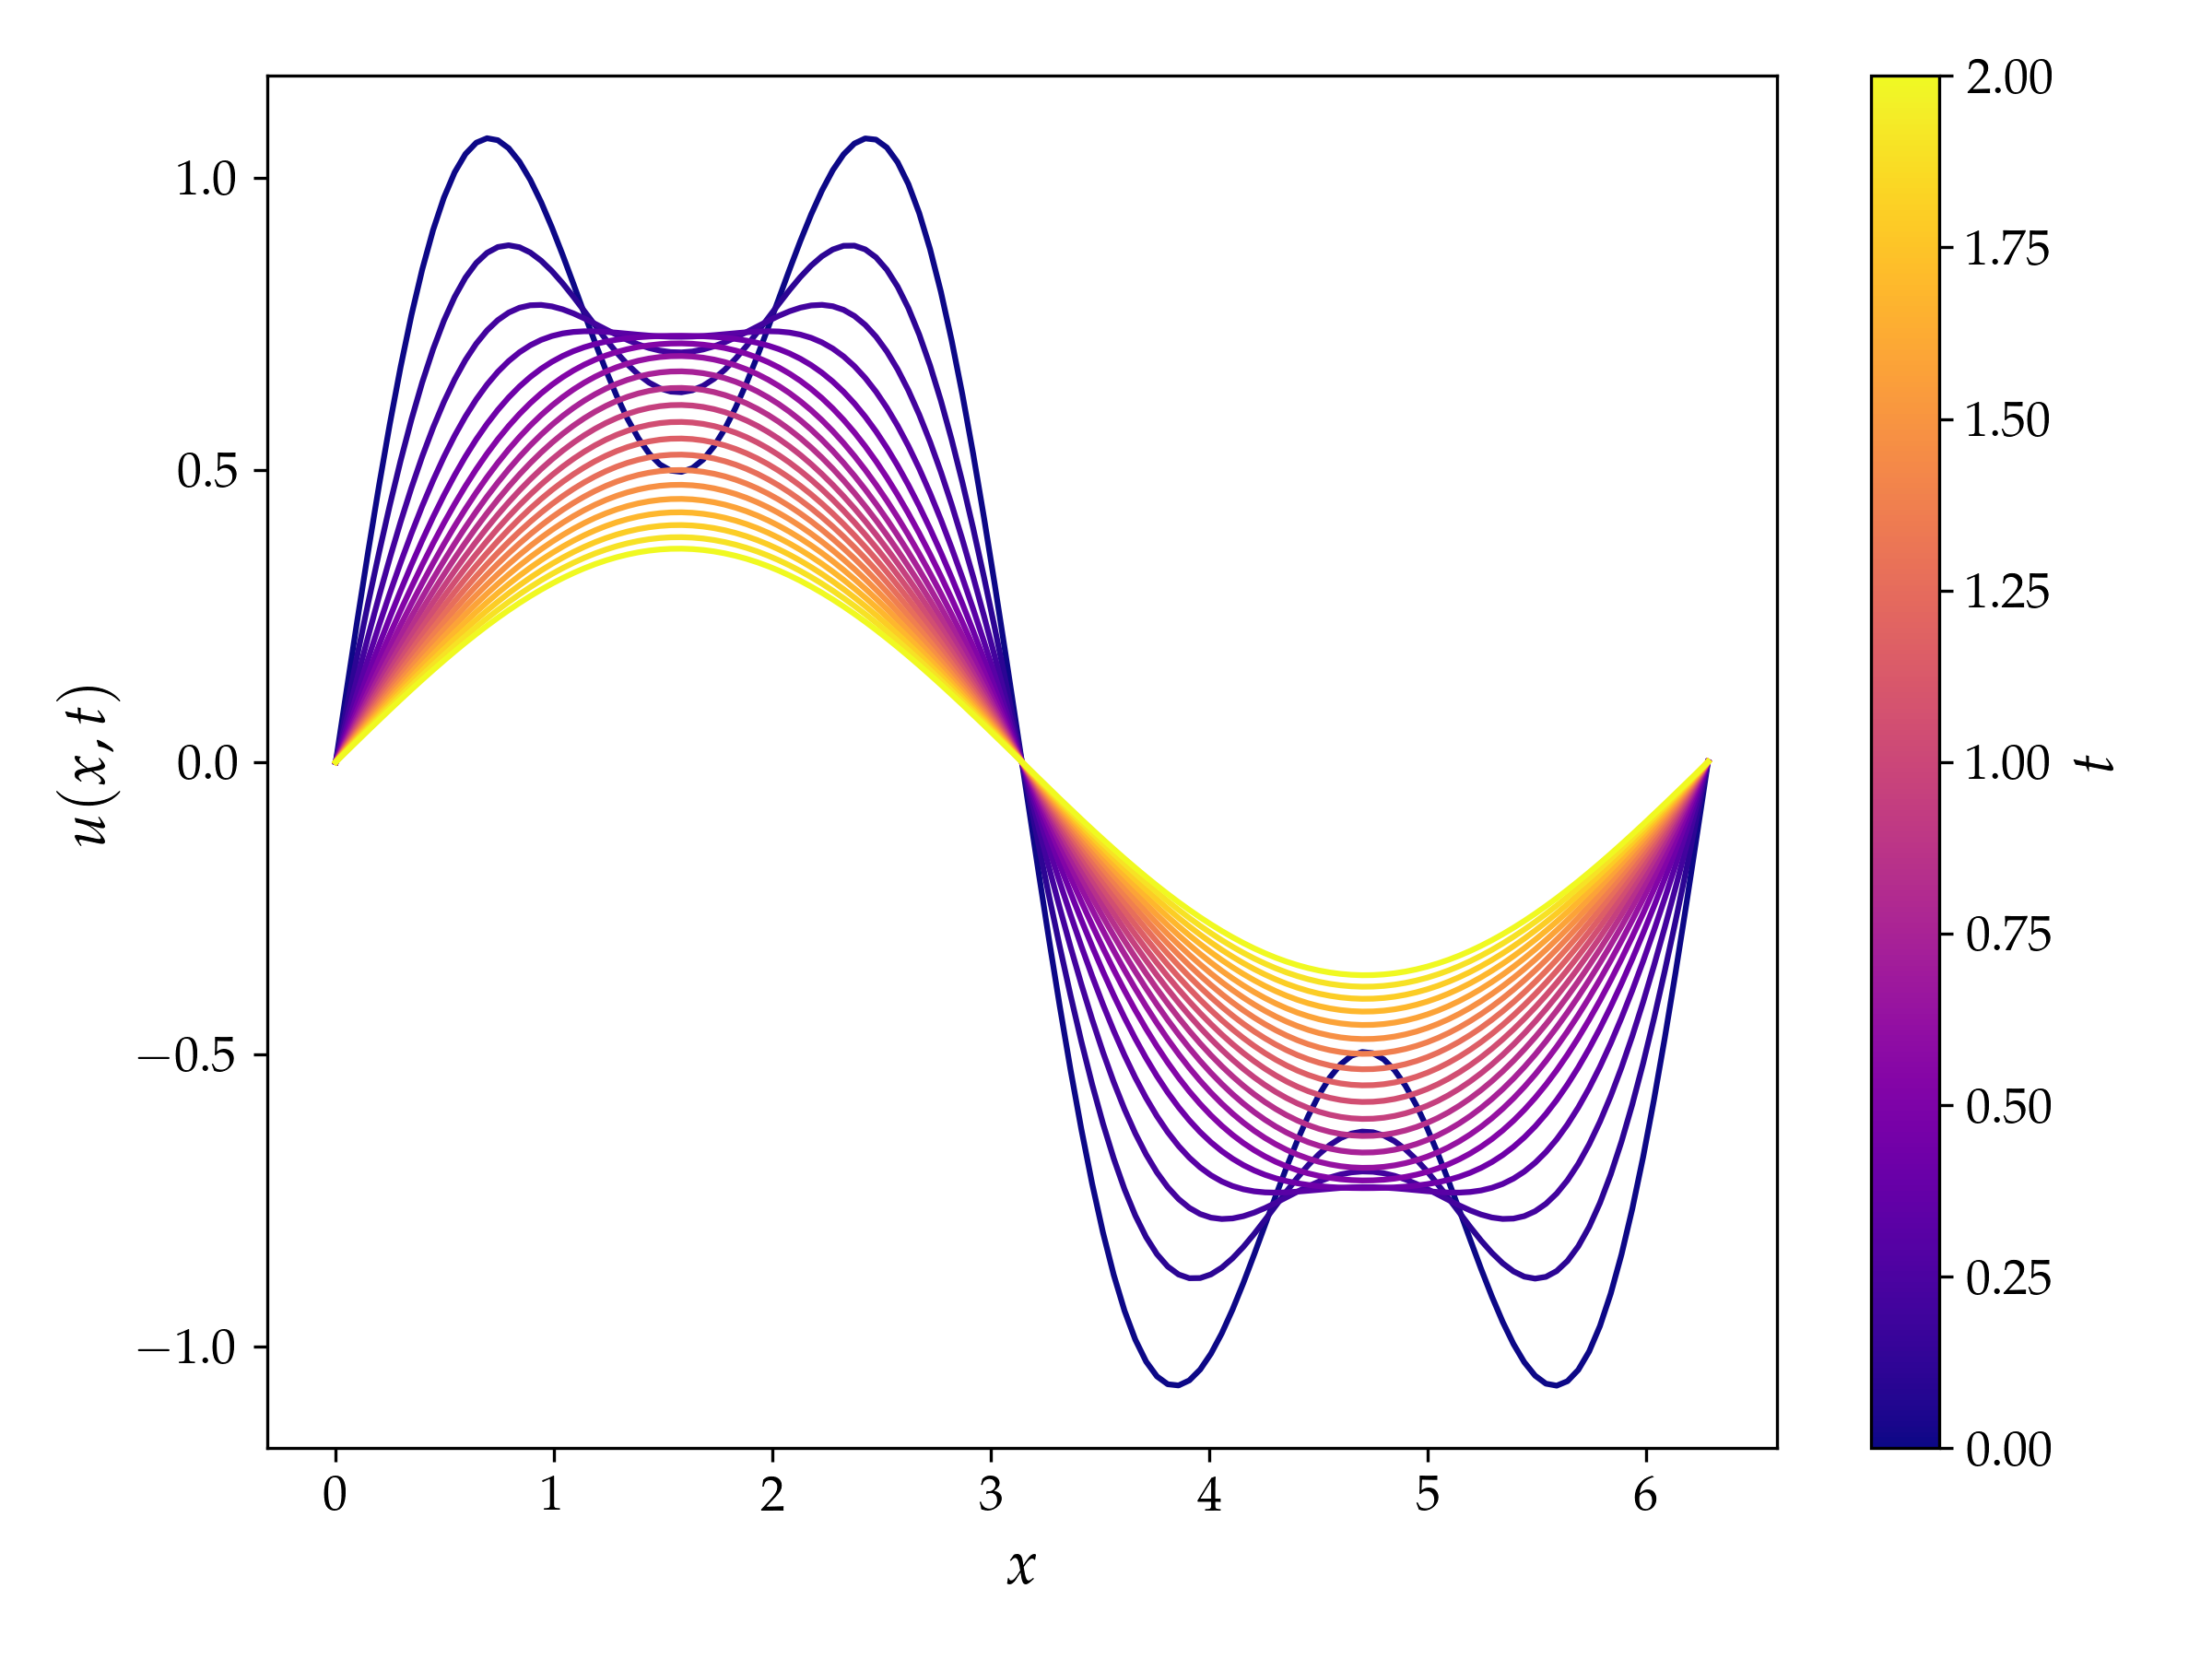
\includegraphics[width=0.8\linewidth]{images/10/heat_sol.png}
    \caption{Variazione del calore in funzione della posizione (asse x) e del tempo (curva di livello con colore assegnato e riportato in legenda).}
    \label{fig: Heat 2d}
\end{figure}

\begin{figure}[H]
    \centering
    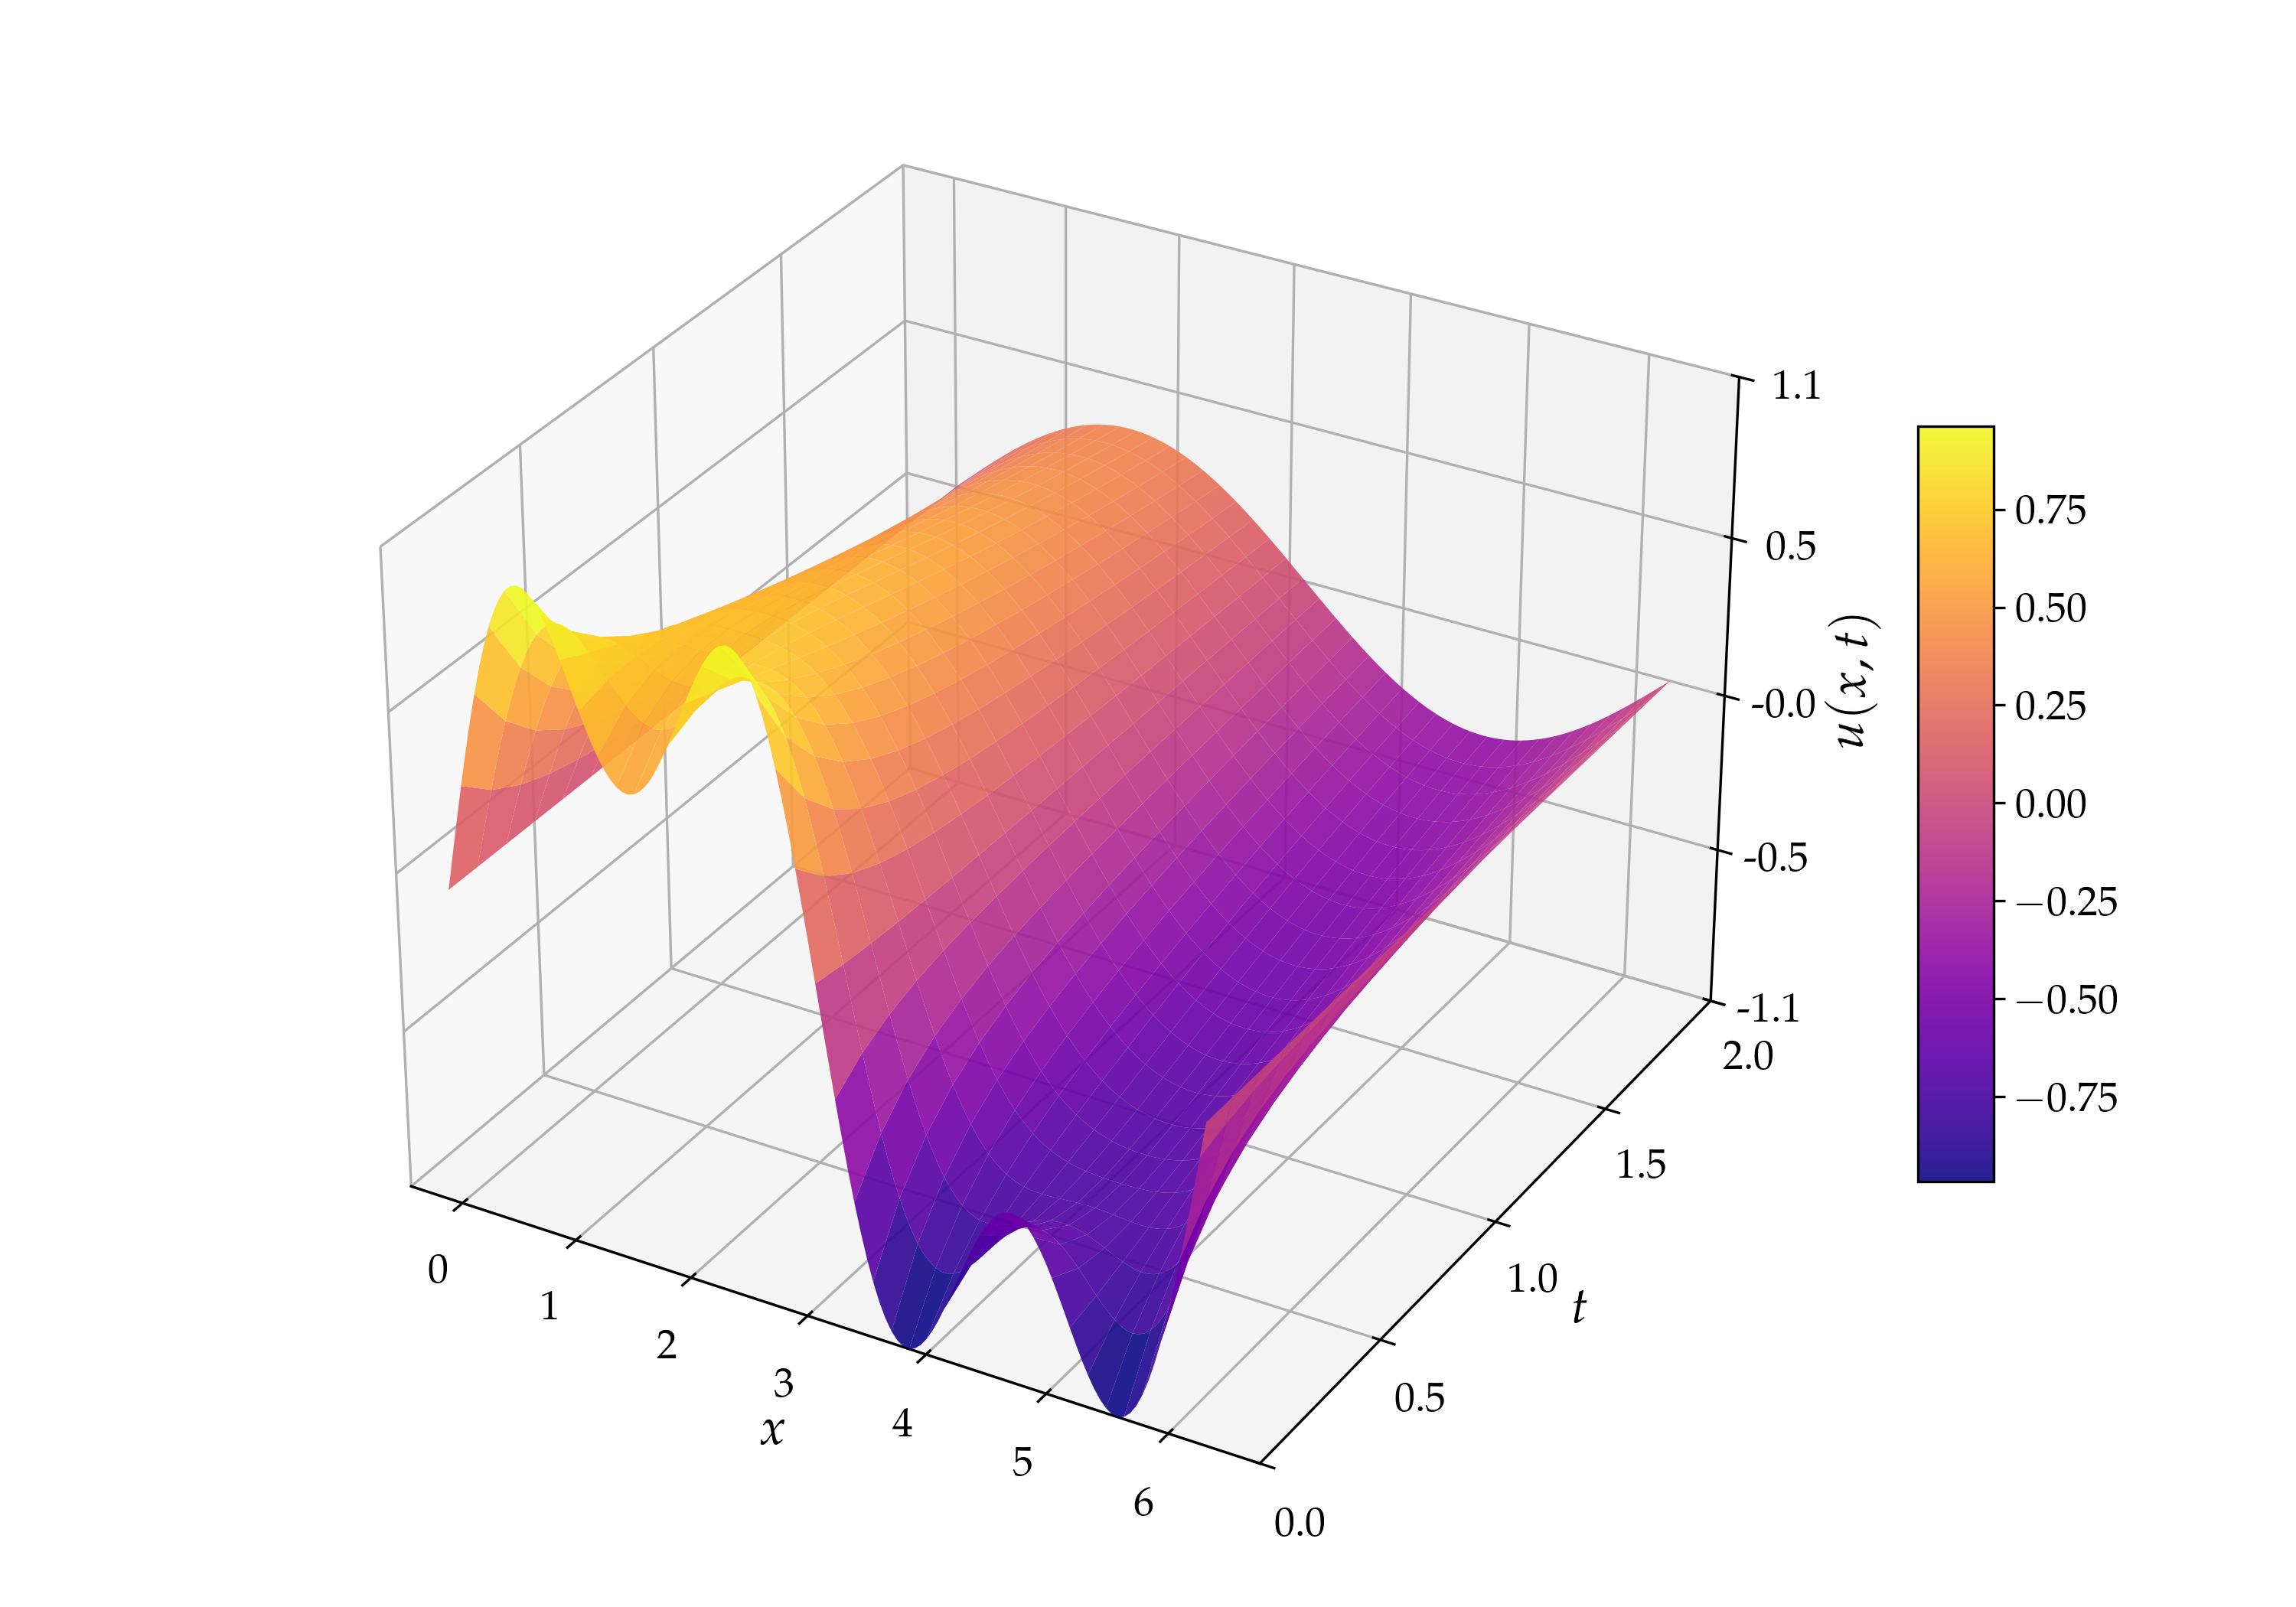
\includegraphics[width=0.8\linewidth]{images/10/heat_sol_3d.png}
    \caption{Variazione del calore in funzione della posizione e tempo con heatmap 3D. Il colore rappresenta il valore della funzione, come riportato in legenda}
    \label{fig: Heat 3d}
\end{figure}

\newpage







\section{Esercizio 4.5.1}
\label{Cap: fitting}
\subsection{Problem Statement}
Scrivi una funzione che accetti $\{x_i\}$, $\{y_i\}$, $C_{ij}$ e $\{f_a\}$ e restituisca il valore del $\chi^2$ insieme ai parametri del fit e ai loro errori.
Quindi testa la funzione sui dati forniti utilizzando
\[
    \frac{F}{(E - M)^2 + \left(\frac{\Gamma}{2}\right)^2}
\]

\noindent Nota che la forma funzionale non è lineare nei parametri ma una semplice trasformazione può renderla tale! Pertanto dovresti procedere come segue:

\begin{enumerate}
    \item trasforma i dati in modo che la funzione di fit sia lineare nella base monomiale. Produci un grafico dei dati trasformati.
    \item esegui il fit sui dati trasformati e calcola i parametri $F, M, \Gamma$ e il $\chi^2$. È un buon fit?
    \item produci un grafico con i dati trasformati e la funzione di fit.
    \item produci il grafico finale con le seguenti caratteristiche:
    \begin{itemize}
        \item i dati originali (con gli errori)
        \item una linea che rappresenta il valore centrale della funzione di fit
        \item \textit{opzionale}: una banda che rappresenta l'errore della funzione di fit ottenuta propagando gli errori dei parametri del fit.
    \end{itemize}
\end{enumerate}

\subsection{Premessa Teorica}
Se il problema dell'interpolazione è in soprattutto un problema di tipo matematico, in questo contesto vogliamo dare la risoluzione di uno fisico. Partendo da un set di due coordinate, di una forma funzionale che ne descrive la relazione, e degli errori che sono associati al valore sperimentale della funzione, è possibile definire un metodo che esegua un'operazione di grande interesse fisico-sperimentale: in particolare si tratta di verificare il grado di compatibilità dell'osservazione con il modello (test $\chi^2$) e calcolare il valore dei parametri liberi che vengono determinati dall'assunzione del modello come valido.

\medskip
Il set di dati è $\boldsymbol{x}_i$ e $\boldsymbol{y}_i$ rappresenta il valore sperimentale della funzione $f(\boldsymbol{x}_i, \boldsymbol{\alpha}_a)$, dove $\boldsymbol{\alpha}_a$ è il vettore dei parametri liberi, quelli che desideriamo stimare con il fit. Se il numero di punti che usiamo per fittare è $N$ e il numero di parametri $N_A$, allora $i = 0, 1, \dots, N-1$  e $a = 0, 1, \dots ,N_A-1$; 
\begin{itemize}
    \item $N = N_A \implies$ Tutti i parametri possono essere fissati esattamente, Fit $\equiv$ Interpolazione.
    \item $N \gg N_A \implies$ È possibile trovare la soluzione migliore minimizzando la norma $\chi^2$:
    $$\chi^2 = [y_i - f(x_i, \boldsymbol{\alpha})] W_{ij} [y_j - f(x_j, \boldsymbol{\alpha})]$$
    la matrice $W$ è quadrata e definita positiva; nel caso di fit con errori sui dati, che sono raccolti nella matrice di covarianza ($C_{ij}$), è utile scegliere $W_{ij}=C_{ij}^{-1}$, poiché questa scelta permette di interpretare il test del $\chi^2$ e il suo \textit{p-val} come significativi della bontà del fit.
\end{itemize}

\subsubsection{La \textit{Normal equation}}
Se è possibile ottenere una funzione lineare nei parametri, è possibile interpretare la risoluzione del problema di fitting come un sistema di equazioni lineari, già discusso nella Parte \ref{Cap: Matrici e Sistemi Lineari}.\\
Definendo $F_i$ come:
\[
F_i = F(x_i) = \sum_{a=0}^{N_a-1} \alpha_a f_a(x_i) =
\sum_{a=0}^{N_a-1} \alpha_a X_{ia}, \quad \quad X_{ia} = f_a(x_i)
\]

\noindent così il residuo nel $\chi^2$ è semplicemente:
\[
    \boldsymbol r =\boldsymbol  y - \boldsymbol  \alpha \, X
\]
\[
\implies \chi^2 = (y^T - \alpha^T X^T) W (y - X\alpha)
\]

$$\xrightarrow{\text{svolgendo}}\chi^2 = y^T Wy - y^T W X\alpha - \alpha^T X^T Wy + \alpha^T X^T W X\alpha$$
$y^T W X \alpha = \alpha^T X^T W^T y$ e assumiamo $W=W^T$, cioè simmetrica: si può riscrivere la relazione precedente come

$$\chi^2 = y^T Wy - 2\alpha^T X^T Wy + \alpha^T X^T W X\alpha$$

\bigskip
\noindent Il nostro algoritmo si basa sulla minimizzazione della metrica $\chi^2$, cioè sul valutare $\frac{\partial \chi^2}{\partial \alpha_a} = 0$. Svolgendo le derivate abbiamo il risultato finale:

$$-2X^T Wy + 2X^T WX\alpha = 0 \quad \longrightarrow{} \quad X^T WX \alpha = X^T Wy$$

Cioè risolvendo per $\alpha$, ipotizzando $M = X^T W X$ invertibile:

$$\alpha = M^{-1} X^T Wy$$

Si può verificare che la matrice di covarianza per i parametri fittati sia:
\[
    C_{ab} = M_{ab}^{-1} \implies \sigma_{\alpha_a} = \sqrt{C_{aa}} 
\]

\subsection{Metodi Numerici e Algoritmi}
\subsubsection{Implementazione della \textit{Decomposizione di Cholesky}}
Notando che $M$ è simmetrica e definita positiva, scegliamo di implementare una risoluzione che faccia uso dell'algoritmo di Cholesky (Cap. \ref{Cap: Cholesky}). Recuperando l'equazione appena trovata possiamo riscrivere in maniera da rendere esplicito il sistema lineare $A \boldsymbol{x} = LL^T\boldsymbol{x}= \boldsymbol{b}$:

\[
    M \boldsymbol \alpha = L L^T \boldsymbol \alpha = X^T W \boldsymbol y = \boldsymbol b
\]

\[
    L \boldsymbol x = \boldsymbol b \,, \quad \to \quad L^T \boldsymbol \alpha = \boldsymbol x
\]

\bigskip
\noindent Nell'appendice \hyperref[App: funzione fit]{App.1} segue una breve digressione sull'implementazione che ho deciso di fare per una funzione specifica per il fit, utile e utilizzata per questo esercizio, ma che ho scelto di usare e generalizzato appositamente anche per diversi utilizzi più avanti nel corso del laboratorio: la funzione fa uso proprio dei metodi descritti in questo paragrafo. 

\subsubsection{Fitting della \textit{Breit-Wigner}}
La funzione che ci è richiesto di fittare non è lineare nel parametro $E$, ma lo può diventare se consideriamo una sua riscrittura, quindi:

\[
  \sigma_{BW}(E) = \frac{F}{(E - M)^2 + \left(\frac{\Gamma}{2}\right)^2} \quad \to \quad
  f(E) = 1 / \sigma_{BW}(E) = aE^2 + bE + c 
\]

\noindent dove $a,b,c$ diventano i nuovi parametri del fit lineare, da cui sapremo poi ricavare i parametri originali della \textit{BW} come:
\[
F = 1/a \quad \quad
M = -\frac{b}{2a} \quad \quad
\Gamma = \frac{\sqrt{4ac - b^2}}{a}
\]

\bigskip

\noindent Nella Fig. \ref{fig: Lin_vsNLin} si può osservare il confronto tra le due curve, $\sigma_{BW}(E)$ e $f(E)$; interessante la maniera in cui si trasformano anche gli errori sui punti, che derivano nel plot a sx dalla matrice di covarianza originale, mentre nel plot di dx dalla propagazione dell'errore su $f=1/\sigma$.

\begin{figure}[H]
    \centering
    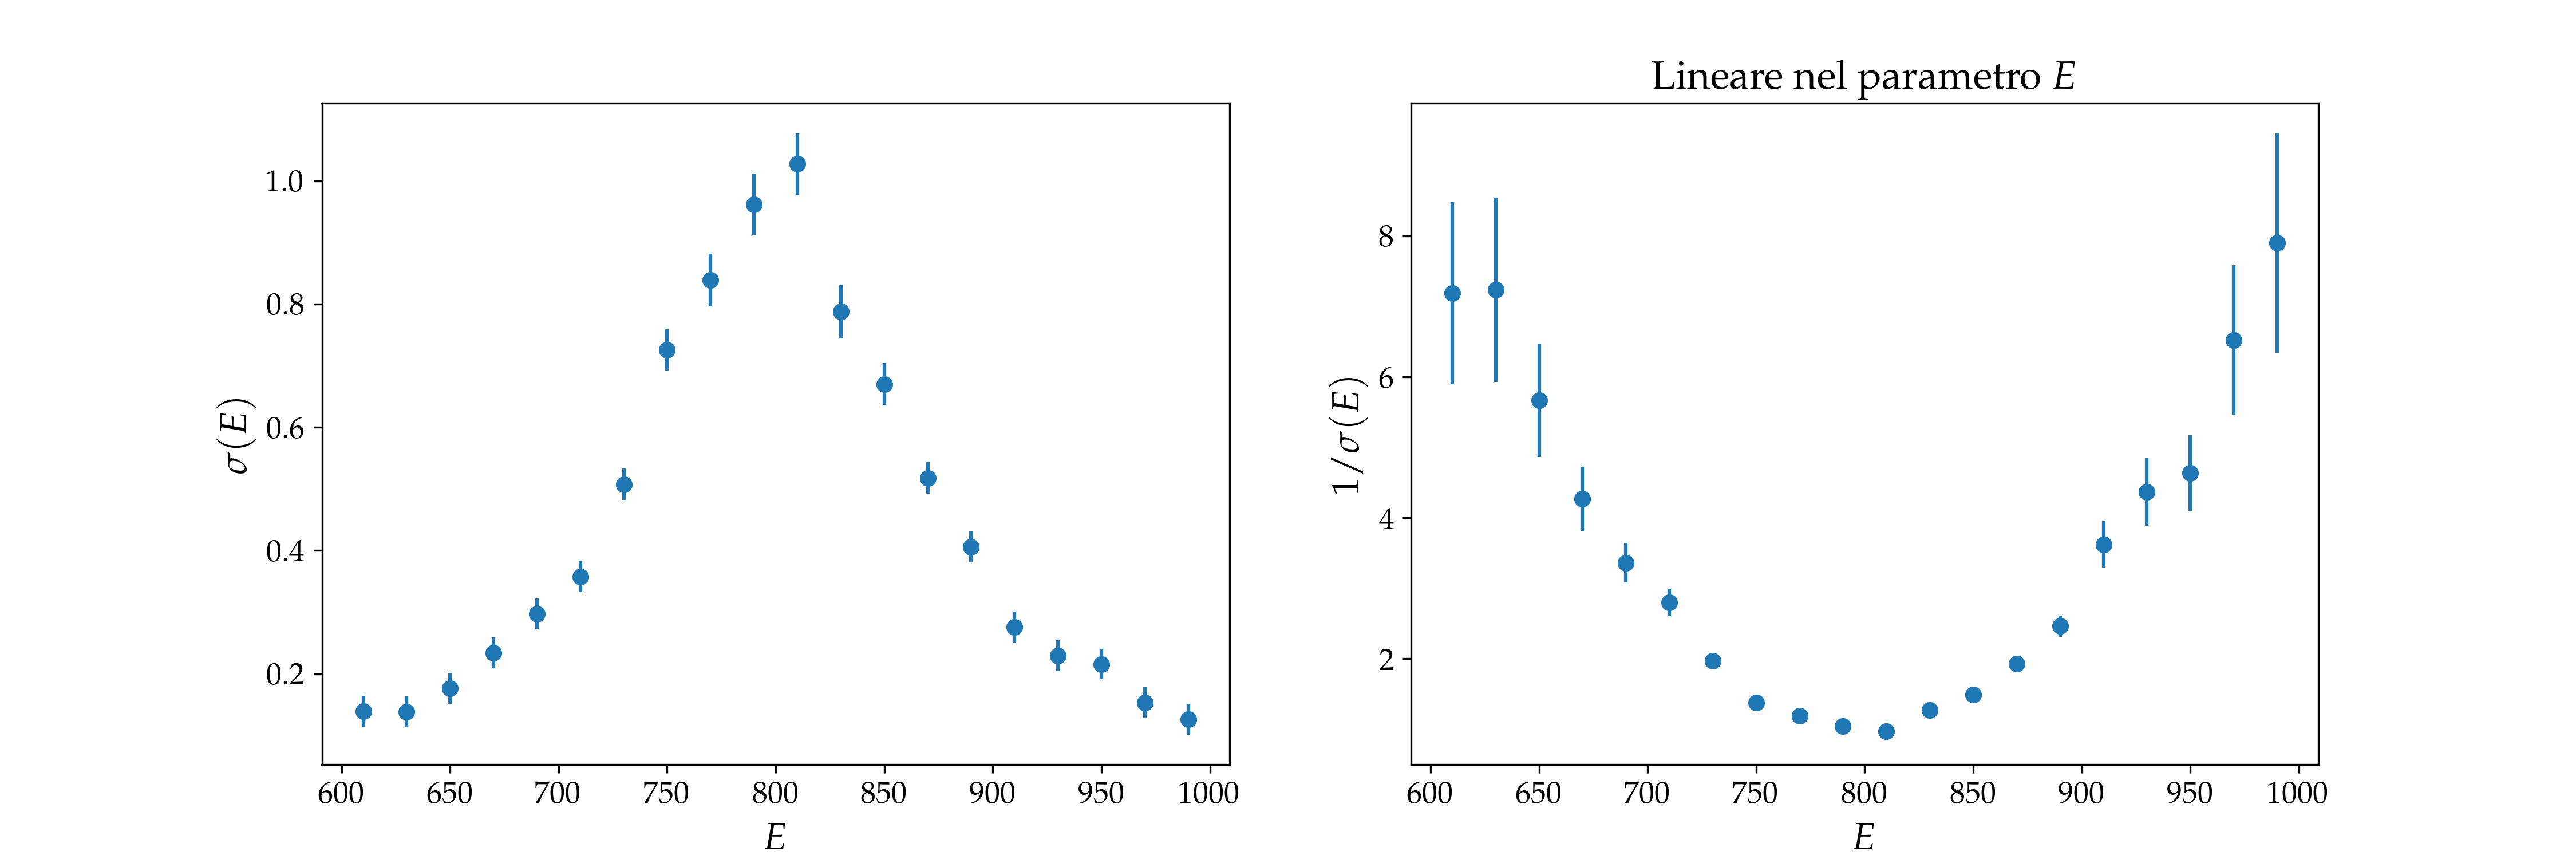
\includegraphics[width=\linewidth]{images/11/confr_lin_nonLin.png}
    \caption{Confronto tra la \textit{BW} e la sua linearizzata.}
    \label{fig: Lin_vsNLin}
\end{figure}


\subsection{Risultati e Discussione}
Esponiamo qui i risultati del fit: partendo dai dati e matrice di covarianza forniti dall'esercizio, procediamo ricavando in primis la matrice di covarianza della funzione linearizzata:
\[
C_{ij}^{(f)} = \frac{\partial f_i}{\partial \sigma_i} C_{ij}^{(\sigma)} \frac{\partial f_j}{\partial \sigma_j} = \frac{1}{\sigma_i^2} C_{ij}^{(\sigma)} \frac{1}{\sigma_j^2}
\]

\noindent Data questa è possibile fittare le $x_i= E_{data}$ con $y_i = \sigma_{data}$, tramite la funzione $f(E)$, già definita precedentemente. Il fit ha queste caratteristiche:
\begin{itemize}
    \item I parametri ottenuti dal fit sono i seguenti:
\begin{center}
    $a = (1.88 \pm 0.10)\times 10^{-4} \text{ MeV}^{-2}$ \\
    \smallskip
    $b = (-3.01 \pm 0.17)\times 10^{-1} \text{ MeV}^{-1}$ \\
    \smallskip
    $c = (1.21 \pm 0.07)\times 10^{2}$
\end{center}
    \item $\chi^2 = 13.5$ ed un corrispondente \textit{p-val($\chi^2$, $\nu$=N-$3$=$17$)} $\approx0.70 \gg 0.05$. I dati hanno una buona aderenza alla funzione $f(E)$ e concludiamo che il fit è buono.

\begin{figure}[H]
    \centering
    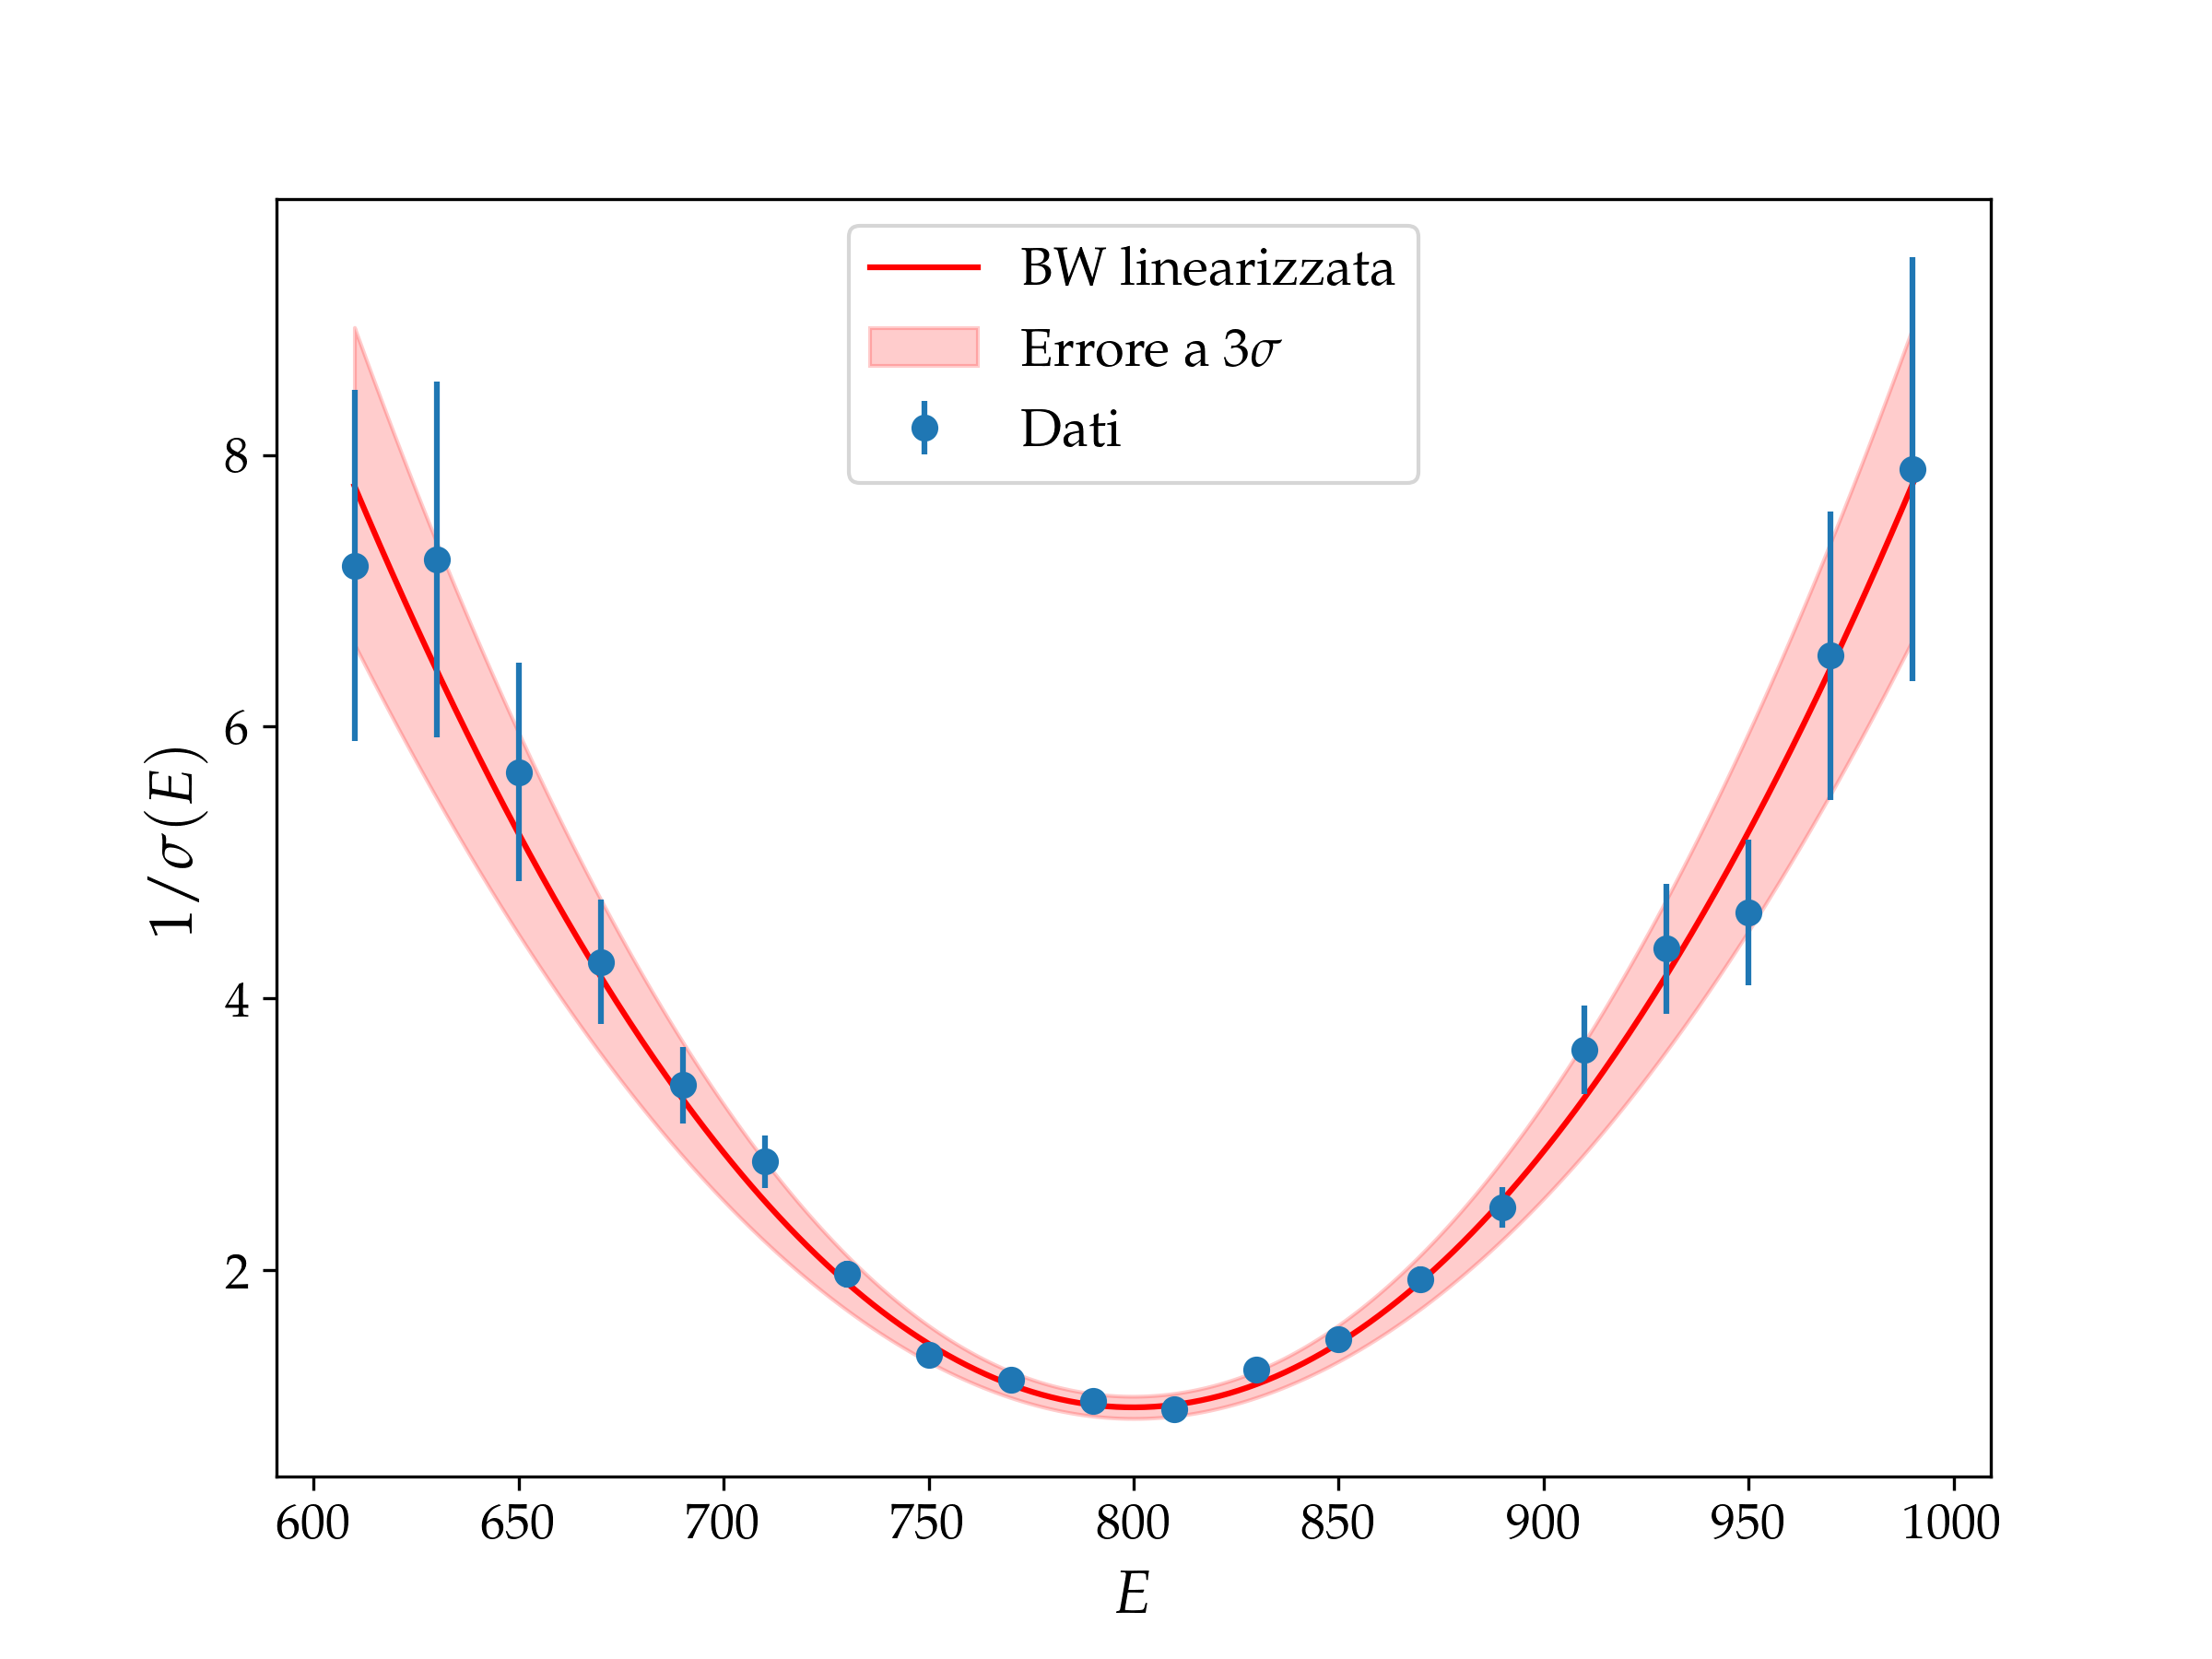
\includegraphics[width=0.68\linewidth]{images/11/Lin_plot.png}
    \caption{Fit della funzione linearizzata, $f(E)$, con errori sui punti e fascia di confidenza a $3\sigma$.}
    \label{fig: Lin_fit}
\end{figure}


    \item Ora possiamo passare ai parametri originali fisici, $F, M, \Gamma$ ed è possibile calcolare i loro errori:
    
\begin{center}
$F = (5.32 \pm 0.29)\times 10^{3} \text{ MeV}^{2}$ \\
\smallskip
$M = (799.9 \pm 1.2) \text{ MeV}$ \\
\smallskip
$\Gamma = (145.1 \pm 5.2) \text{ MeV}$
\end{center}

Possiamo evidenziare la coerenza con quelli che lo statement suggerisce come veri\\($M_{true}=800$ Mev, $\Gamma_{true}=140$ Mev), usati per la generazione del sample.

\begin{figure}[H]
    \centering
    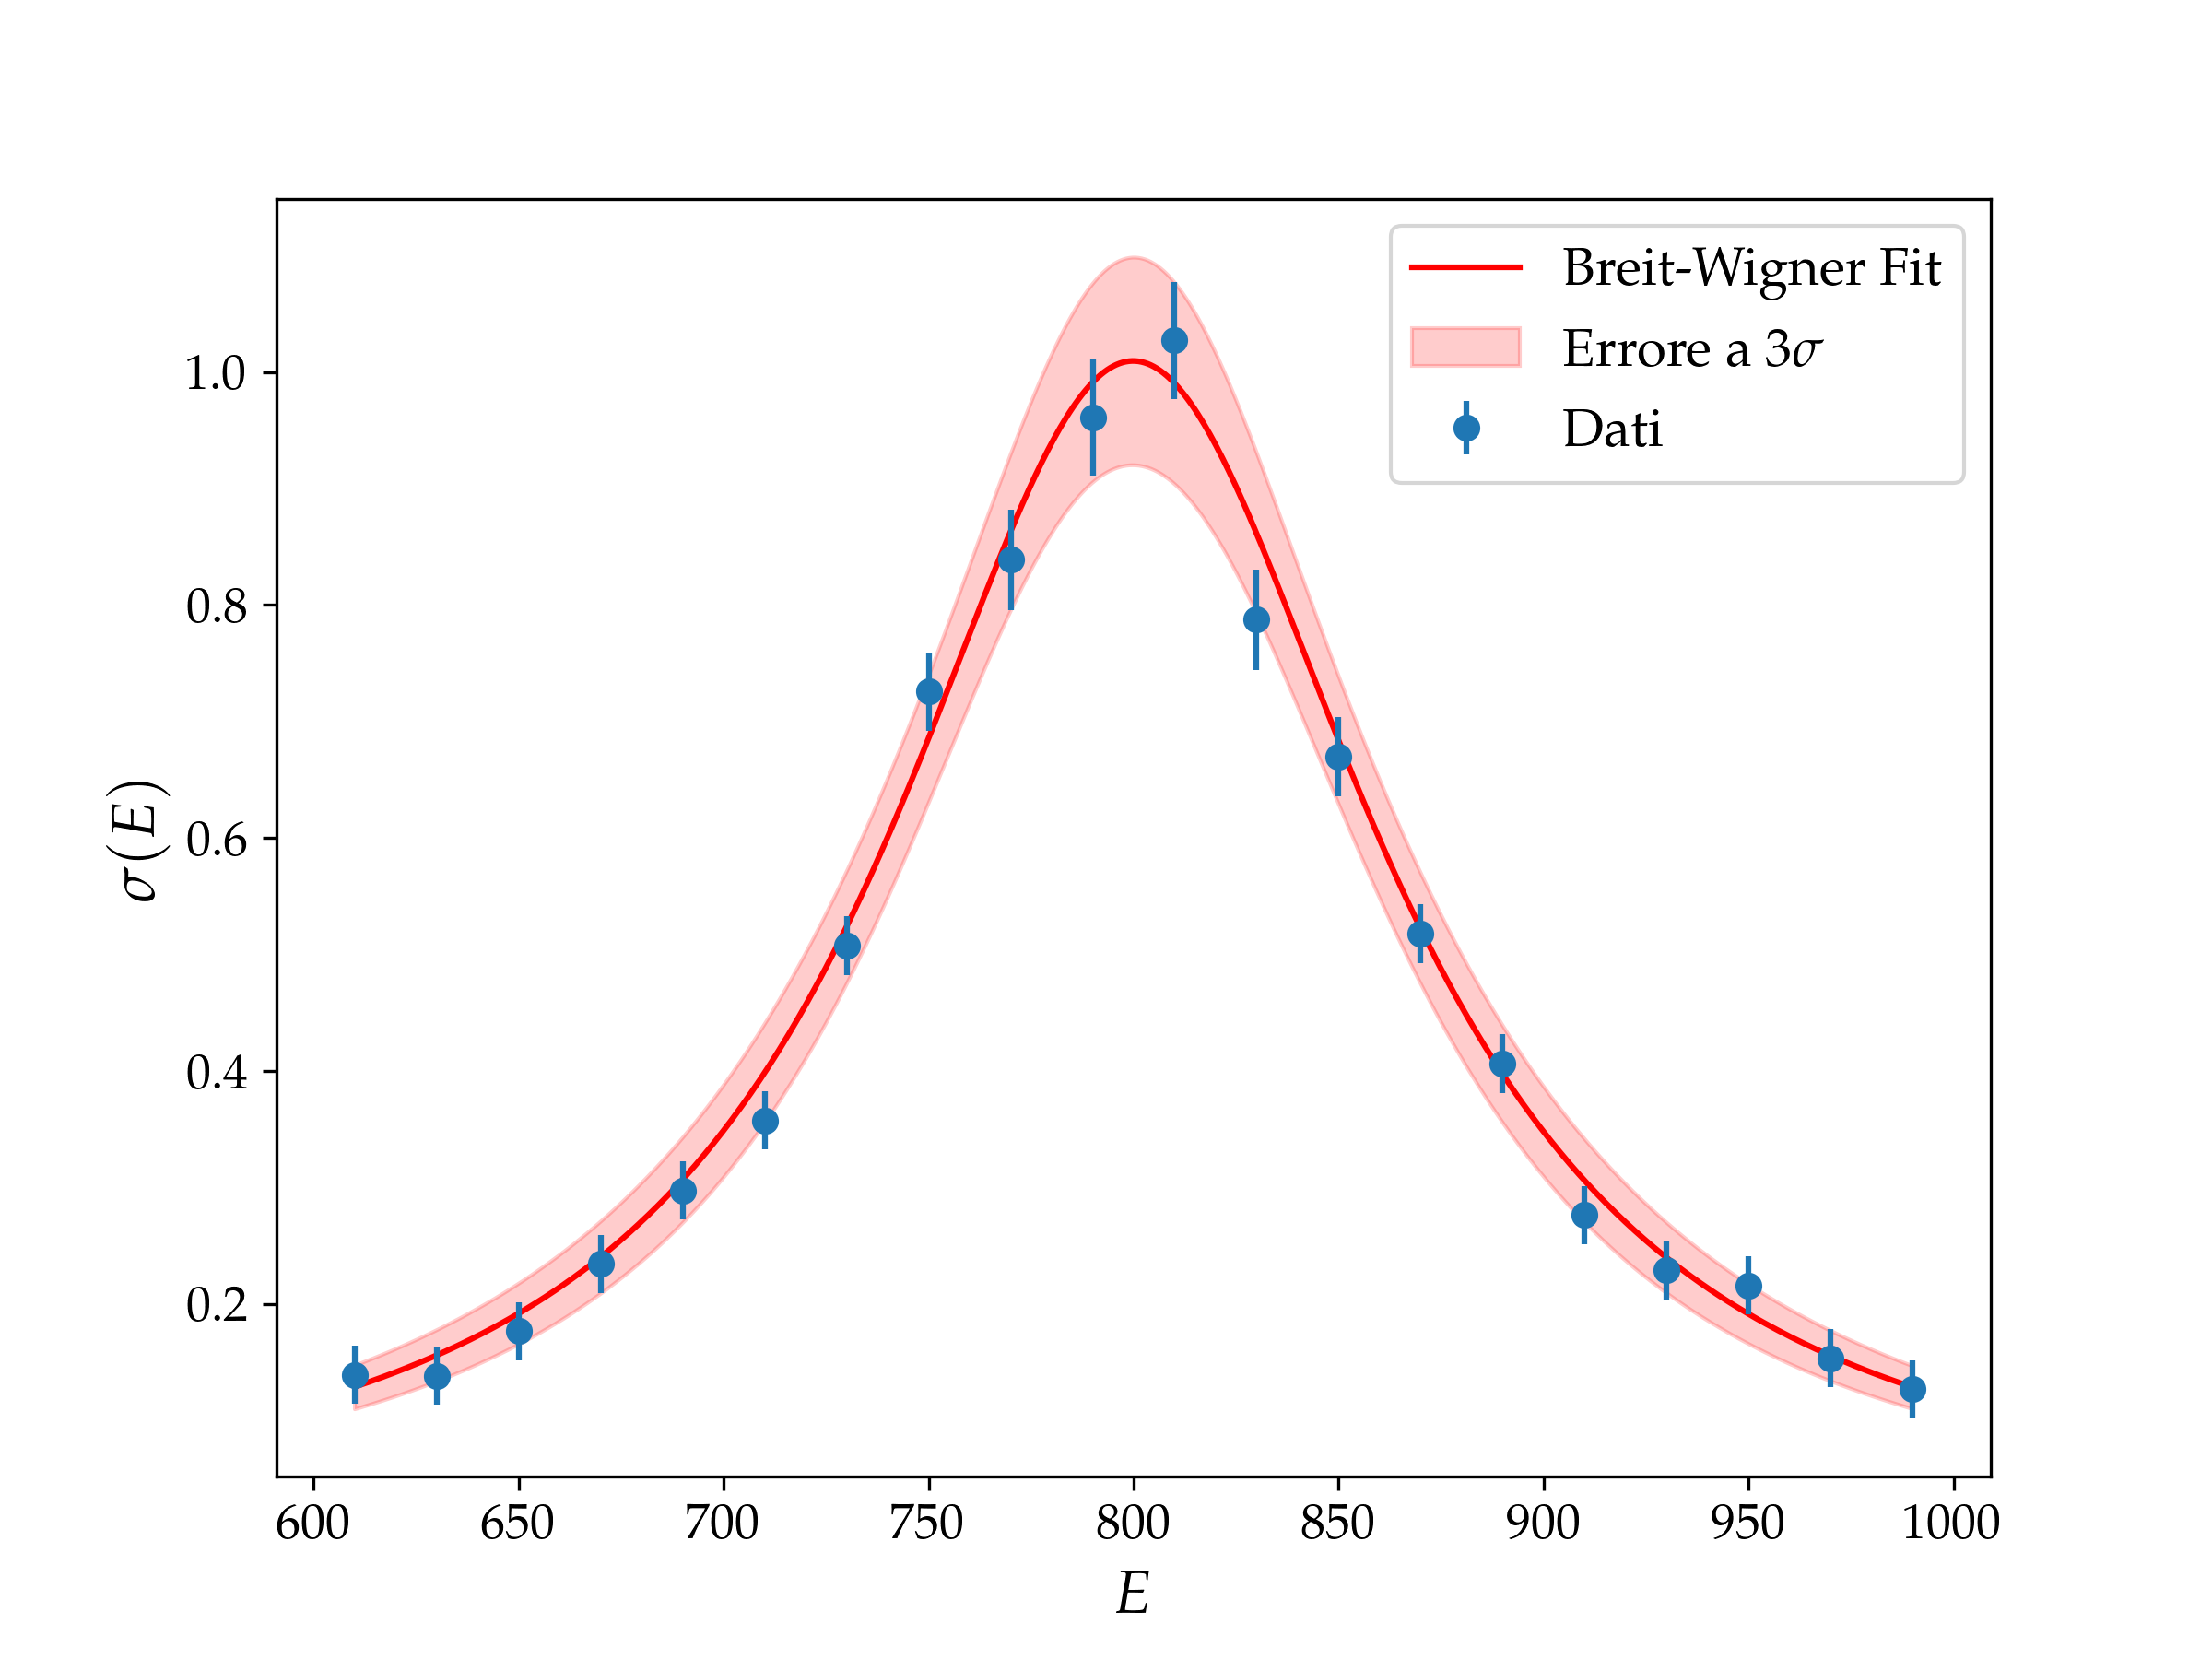
\includegraphics[width=0.68\linewidth]{images/11/Scatt_plot.png}
    \caption{Fit della \textit{Breit-Wigner}, $\sigma_{BW}(E)$, con errori sui punti e fascia di confidenza a $3\sigma$.}
    \label{fig: BW_fit}
\end{figure}
\end{itemize}

